\documentclass[twoside]{book}

% Packages required by doxygen
\usepackage{calc}
\usepackage{doxygen}
\usepackage{graphicx}
\usepackage[utf8]{inputenc}
\usepackage{makeidx}
\usepackage{multicol}
\usepackage{multirow}
\usepackage{textcomp}
\usepackage[table]{xcolor}

% NLS support packages
\usepackage{polski}
\usepackage[T1]{fontenc}

% Font selection
\usepackage[T1]{fontenc}
\usepackage{mathptmx}
\usepackage[scaled=.90]{helvet}
\usepackage{courier}
\usepackage{amssymb}
\usepackage{sectsty}
\renewcommand{\familydefault}{\sfdefault}
\allsectionsfont{%
  \fontseries{bc}\selectfont%
  \color{darkgray}%
}
\renewcommand{\DoxyLabelFont}{%
  \fontseries{bc}\selectfont%
  \color{darkgray}%
}

% Page & text layout
\usepackage{geometry}
\geometry{%
  a4paper,%
  top=2.5cm,%
  bottom=2.5cm,%
  left=2.5cm,%
  right=2.5cm%
}
\tolerance=750
\hfuzz=15pt
\hbadness=750
\setlength{\emergencystretch}{15pt}
\setlength{\parindent}{0cm}
\setlength{\parskip}{0.2cm}
\makeatletter
\renewcommand{\paragraph}{%
  \@startsection{paragraph}{4}{0ex}{-1.0ex}{1.0ex}{%
    \normalfont\normalsize\bfseries\SS@parafont%
  }%
}
\renewcommand{\subparagraph}{%
  \@startsection{subparagraph}{5}{0ex}{-1.0ex}{1.0ex}{%
    \normalfont\normalsize\bfseries\SS@subparafont%
  }%
}
\makeatother

% Headers & footers
\usepackage{fancyhdr}
\pagestyle{fancyplain}
\fancyhead[LE]{\fancyplain{}{\bfseries\thepage}}
\fancyhead[CE]{\fancyplain{}{}}
\fancyhead[RE]{\fancyplain{}{\bfseries\leftmark}}
\fancyhead[LO]{\fancyplain{}{\bfseries\rightmark}}
\fancyhead[CO]{\fancyplain{}{}}
\fancyhead[RO]{\fancyplain{}{\bfseries\thepage}}
\fancyfoot[LE]{\fancyplain{}{}}
\fancyfoot[CE]{\fancyplain{}{}}
\fancyfoot[RE]{\fancyplain{}{\bfseries\scriptsize Wygenerowano So, 4 sty 2014 10\-:40\-:17 dla Projekt szachowy programem Doxygen }}
\fancyfoot[LO]{\fancyplain{}{\bfseries\scriptsize Wygenerowano So, 4 sty 2014 10\-:40\-:17 dla Projekt szachowy programem Doxygen }}
\fancyfoot[CO]{\fancyplain{}{}}
\fancyfoot[RO]{\fancyplain{}{}}
\renewcommand{\footrulewidth}{0.4pt}
\renewcommand{\chaptermark}[1]{%
  \markboth{#1}{}%
}
\renewcommand{\sectionmark}[1]{%
  \markright{\thesection\ #1}%
}

% Indices & bibliography
\usepackage{natbib}
\usepackage[titles]{tocloft}
\setcounter{tocdepth}{3}
\setcounter{secnumdepth}{5}
\makeindex

% Hyperlinks (required, but should be loaded last)
\usepackage{ifpdf}
\ifpdf
  \usepackage[pdftex,pagebackref=true]{hyperref}
\else
  \usepackage[ps2pdf,pagebackref=true]{hyperref}
\fi
\hypersetup{%
  colorlinks=true,%
  linkcolor=blue,%
  citecolor=blue,%
  unicode%
}

% Custom commands
\newcommand{\clearemptydoublepage}{%
  \newpage{\pagestyle{empty}\cleardoublepage}%
}


%===== C O N T E N T S =====

\begin{document}

% Titlepage & ToC
\hypersetup{pageanchor=false}
\pagenumbering{roman}
\begin{titlepage}
\vspace*{7cm}
\begin{center}%
{\Large Projekt szachowy }\\
\vspace*{1cm}
{\large Wygenerowano przez Doxygen 1.8.5}\\
\vspace*{0.5cm}
{\small So, 4 sty 2014 10:40:17}\\
\end{center}
\end{titlepage}
\clearemptydoublepage
\tableofcontents
\clearemptydoublepage
\pagenumbering{arabic}
\hypersetup{pageanchor=true}

%--- Begin generated contents ---
\chapter{Indeks przestrzeni nazw}
\section{Pakiety}
Oto lista pakietów wraz z krótkim opisem (o ile jest dostępny)\-:\begin{DoxyCompactList}
\item\contentsline{section}{\hyperlink{namespace_basic_blue}{Basic\-Blue} }{\pageref{namespace_basic_blue}}{}
\item\contentsline{section}{\hyperlink{namespace_basic_blue_1_1_properties}{Basic\-Blue.\-Properties} }{\pageref{namespace_basic_blue_1_1_properties}}{}
\item\contentsline{section}{\hyperlink{namespace_szachy_basic_blue}{Szachy\-Basic\-Blue} }{\pageref{namespace_szachy_basic_blue}}{}
\end{DoxyCompactList}

\chapter{Indeks hierarchiczny}
\section{Hierarchia klas}
Ta lista dziedziczenia posortowana jest z grubsza, choć nie całkowicie, alfabetycznie\-:\begin{DoxyCompactList}
\item Application\-Settings\-Base\begin{DoxyCompactList}
\item \contentsline{section}{Basic\-Blue.\-Properties.\-Settings}{\pageref{class_basic_blue_1_1_properties_1_1_settings}}{}
\end{DoxyCompactList}
\item \contentsline{section}{Szachy\-Basic\-Blue.\-Bierka}{\pageref{class_szachy_basic_blue_1_1_bierka}}{}
\begin{DoxyCompactList}
\item \contentsline{section}{Szachy\-Basic\-Blue.\-Goniec}{\pageref{class_szachy_basic_blue_1_1_goniec}}{}
\item \contentsline{section}{Szachy\-Basic\-Blue.\-Hetman}{\pageref{class_szachy_basic_blue_1_1_hetman}}{}
\item \contentsline{section}{Szachy\-Basic\-Blue.\-Kr�l}{\pageref{class_szachy_basic_blue_1_1_kr_xF3l}}{}
\item \contentsline{section}{Szachy\-Basic\-Blue.\-Pionek}{\pageref{class_szachy_basic_blue_1_1_pionek}}{}
\item \contentsline{section}{Szachy\-Basic\-Blue.\-Skoczek}{\pageref{class_szachy_basic_blue_1_1_skoczek}}{}
\item \contentsline{section}{Szachy\-Basic\-Blue.\-Wie�a}{\pageref{class_szachy_basic_blue_1_1_wie_xBFa}}{}
\end{DoxyCompactList}
\item Form\begin{DoxyCompactList}
\item \contentsline{section}{Basic\-Blue.\-Form1}{\pageref{class_basic_blue_1_1_form1}}{}
\end{DoxyCompactList}
\item \contentsline{section}{Szachy\-Basic\-Blue.\-Historia\-\_\-\-Ruch�w}{\pageref{class_szachy_basic_blue_1_1_historia___ruch_xF3w}}{}
\item \contentsline{section}{Szachy\-Basic\-Blue.\-Odczyt\-Gry}{\pageref{class_szachy_basic_blue_1_1_odczyt_gry}}{}
\item \contentsline{section}{Szachy\-Basic\-Blue.\-Pionki\-\_\-\-Gracza}{\pageref{class_szachy_basic_blue_1_1_pionki___gracza}}{}
\item \contentsline{section}{Szachy\-Basic\-Blue.\-Presti�}{\pageref{class_szachy_basic_blue_1_1_presti_xBF}}{}
\item \contentsline{section}{Basic\-Blue.\-Properties.\-Resources}{\pageref{class_basic_blue_1_1_properties_1_1_resources}}{}
\item \contentsline{section}{Szachy\-Basic\-Blue.\-Silnik\-\_\-\-Gracza}{\pageref{interface_szachy_basic_blue_1_1_silnik___gracza}}{}
\begin{DoxyCompactList}
\item \contentsline{section}{Szachy\-Basic\-Blue.\-Cz�owiek}{\pageref{class_szachy_basic_blue_1_1_cz_xB3owiek}}{}
\item \contentsline{section}{Szachy\-Basic\-Blue.\-Gracz}{\pageref{class_szachy_basic_blue_1_1_gracz}}{}
\item \contentsline{section}{Szachy\-Basic\-Blue.\-Komputer}{\pageref{class_szachy_basic_blue_1_1_komputer}}{}
\end{DoxyCompactList}
\item \contentsline{section}{Szachy\-Basic\-Blue.\-Szachownica}{\pageref{class_szachy_basic_blue_1_1_szachownica}}{}
\item Wynik\-Gry\begin{DoxyCompactList}
\item \contentsline{section}{Szachy\-Basic\-Blue.\-Gra}{\pageref{class_szachy_basic_blue_1_1_gra}}{}
\end{DoxyCompactList}
\item \contentsline{section}{Szachy\-Basic\-Blue.\-Zapis\-Gry}{\pageref{class_szachy_basic_blue_1_1_zapis_gry}}{}
\end{DoxyCompactList}

\chapter{Indeks klas}
\section{Lista klas}
Tutaj znajdują się klasy, struktury, unie i interfejsy wraz z ich krótkimi opisami\-:\begin{DoxyCompactList}
\item\contentsline{section}{\hyperlink{class_szachy_basic_blue_1_1_bierka}{Szachy\-Basic\-Blue.\-Bierka} \\*Klasa s�u�y do pokazania u�ytkownikowi dost�pnych ruch�w figur i obliczenie najlepszego ruchu. Klasa pokazuje nam r�wnie� ilo�� dost�pnych porusze� figur. Wybiera najlepszy ruch. }{\pageref{class_szachy_basic_blue_1_1_bierka}}{}
\item\contentsline{section}{\hyperlink{class_szachy_basic_blue_1_1_cz_xB3owiek}{Szachy\-Basic\-Blue.\-Cz�owiek} }{\pageref{class_szachy_basic_blue_1_1_cz_xB3owiek}}{}
\item\contentsline{section}{\hyperlink{class_basic_blue_1_1_form1}{Basic\-Blue.\-Form1} }{\pageref{class_basic_blue_1_1_form1}}{}
\item\contentsline{section}{\hyperlink{class_szachy_basic_blue_1_1_goniec}{Szachy\-Basic\-Blue.\-Goniec} }{\pageref{class_szachy_basic_blue_1_1_goniec}}{}
\item\contentsline{section}{\hyperlink{class_szachy_basic_blue_1_1_gra}{Szachy\-Basic\-Blue.\-Gra} }{\pageref{class_szachy_basic_blue_1_1_gra}}{}
\item\contentsline{section}{\hyperlink{class_szachy_basic_blue_1_1_gracz}{Szachy\-Basic\-Blue.\-Gracz} }{\pageref{class_szachy_basic_blue_1_1_gracz}}{}
\item\contentsline{section}{\hyperlink{class_szachy_basic_blue_1_1_hetman}{Szachy\-Basic\-Blue.\-Hetman} }{\pageref{class_szachy_basic_blue_1_1_hetman}}{}
\item\contentsline{section}{\hyperlink{class_szachy_basic_blue_1_1_historia___ruch_xF3w}{Szachy\-Basic\-Blue.\-Historia\-\_\-\-Ruch�w} }{\pageref{class_szachy_basic_blue_1_1_historia___ruch_xF3w}}{}
\item\contentsline{section}{\hyperlink{class_szachy_basic_blue_1_1_komputer}{Szachy\-Basic\-Blue.\-Komputer} }{\pageref{class_szachy_basic_blue_1_1_komputer}}{}
\item\contentsline{section}{\hyperlink{class_szachy_basic_blue_1_1_kr_xF3l}{Szachy\-Basic\-Blue.\-Kr�l} }{\pageref{class_szachy_basic_blue_1_1_kr_xF3l}}{}
\item\contentsline{section}{\hyperlink{class_szachy_basic_blue_1_1_odczyt_gry}{Szachy\-Basic\-Blue.\-Odczyt\-Gry} }{\pageref{class_szachy_basic_blue_1_1_odczyt_gry}}{}
\item\contentsline{section}{\hyperlink{class_szachy_basic_blue_1_1_pionek}{Szachy\-Basic\-Blue.\-Pionek} }{\pageref{class_szachy_basic_blue_1_1_pionek}}{}
\item\contentsline{section}{\hyperlink{class_szachy_basic_blue_1_1_pionki___gracza}{Szachy\-Basic\-Blue.\-Pionki\-\_\-\-Gracza} }{\pageref{class_szachy_basic_blue_1_1_pionki___gracza}}{}
\item\contentsline{section}{\hyperlink{class_szachy_basic_blue_1_1_presti_xBF}{Szachy\-Basic\-Blue.\-Presti�} \\*Nadanie presti�u wszystkim figurom }{\pageref{class_szachy_basic_blue_1_1_presti_xBF}}{}
\item\contentsline{section}{\hyperlink{class_basic_blue_1_1_properties_1_1_resources}{Basic\-Blue.\-Properties.\-Resources} \\*A strongly-\/typed resource class, for looking up localized strings, etc. }{\pageref{class_basic_blue_1_1_properties_1_1_resources}}{}
\item\contentsline{section}{\hyperlink{class_basic_blue_1_1_properties_1_1_settings}{Basic\-Blue.\-Properties.\-Settings} }{\pageref{class_basic_blue_1_1_properties_1_1_settings}}{}
\item\contentsline{section}{\hyperlink{interface_szachy_basic_blue_1_1_silnik___gracza}{Szachy\-Basic\-Blue.\-Silnik\-\_\-\-Gracza} }{\pageref{interface_szachy_basic_blue_1_1_silnik___gracza}}{}
\item\contentsline{section}{\hyperlink{class_szachy_basic_blue_1_1_skoczek}{Szachy\-Basic\-Blue.\-Skoczek} }{\pageref{class_szachy_basic_blue_1_1_skoczek}}{}
\item\contentsline{section}{\hyperlink{class_szachy_basic_blue_1_1_szachownica}{Szachy\-Basic\-Blue.\-Szachownica} }{\pageref{class_szachy_basic_blue_1_1_szachownica}}{}
\item\contentsline{section}{\hyperlink{class_szachy_basic_blue_1_1_wie_xBFa}{Szachy\-Basic\-Blue.\-Wie�a} }{\pageref{class_szachy_basic_blue_1_1_wie_xBFa}}{}
\item\contentsline{section}{\hyperlink{class_szachy_basic_blue_1_1_zapis_gry}{Szachy\-Basic\-Blue.\-Zapis\-Gry} }{\pageref{class_szachy_basic_blue_1_1_zapis_gry}}{}
\end{DoxyCompactList}

\chapter{Indeks plików}
\section{Lista plików}
Tutaj znajduje się lista wszystkich plików z ich krótkimi opisami\-:\begin{DoxyCompactList}
\item\contentsline{section}{\hyperlink{_assembly_info_8cs}{Assembly\-Info.\-cs} }{\pageref{_assembly_info_8cs}}{}
\item\contentsline{section}{\hyperlink{_bierka_8cs}{Bierka.\-cs} }{\pageref{_bierka_8cs}}{}
\item\contentsline{section}{\hyperlink{_form1_8cs}{Form1.\-cs} }{\pageref{_form1_8cs}}{}
\item\contentsline{section}{\hyperlink{_form1_8_designer_8cs}{Form1.\-Designer.\-cs} }{\pageref{_form1_8_designer_8cs}}{}
\item\contentsline{section}{\hyperlink{_goniec_8cs}{Goniec.\-cs} }{\pageref{_goniec_8cs}}{}
\item\contentsline{section}{\hyperlink{_gra_8cs}{Gra.\-cs} }{\pageref{_gra_8cs}}{}
\item\contentsline{section}{\hyperlink{_gracz-_cz_xC5_x82owiek_8cs}{Gracz-\/\-Człowiek.\-cs} }{\pageref{_gracz-_cz_xC5_x82owiek_8cs}}{}
\item\contentsline{section}{\hyperlink{_gracz-_komputer_8cs}{Gracz-\/\-Komputer.\-cs} }{\pageref{_gracz-_komputer_8cs}}{}
\item\contentsline{section}{\hyperlink{_gracz_8cs}{Gracz.\-cs} }{\pageref{_gracz_8cs}}{}
\item\contentsline{section}{\hyperlink{_hetman_8cs}{Hetman.\-cs} }{\pageref{_hetman_8cs}}{}
\item\contentsline{section}{\hyperlink{_historia___ruch_xC3_xB3w_8cs}{Historia\-\_\-\-Ruchów.\-cs} }{\pageref{_historia___ruch_xC3_xB3w_8cs}}{}
\item\contentsline{section}{\hyperlink{_kierunek_ruchu_8cs}{Kierunek\-Ruchu.\-cs} }{\pageref{_kierunek_ruchu_8cs}}{}
\item\contentsline{section}{\hyperlink{_kolor___gracza_8cs}{Kolor\-\_\-\-Gracza.\-cs} }{\pageref{_kolor___gracza_8cs}}{}
\item\contentsline{section}{\hyperlink{_kolor__pionk_xC3_xB3w_8cs}{Kolor\-\_\-pionków.\-cs} }{\pageref{_kolor__pionk_xC3_xB3w_8cs}}{}
\item\contentsline{section}{\hyperlink{_kr_xC3_xB3l_8cs}{Król.\-cs} }{\pageref{_kr_xC3_xB3l_8cs}}{}
\item\contentsline{section}{\hyperlink{_odczyt_gry_8cs}{Odczyt\-Gry.\-cs} }{\pageref{_odczyt_gry_8cs}}{}
\item\contentsline{section}{\hyperlink{_pionek_8cs}{Pionek.\-cs} }{\pageref{_pionek_8cs}}{}
\item\contentsline{section}{\hyperlink{_pionki___gracza_8cs}{Pionki\-\_\-\-Gracza.\-cs} }{\pageref{_pionki___gracza_8cs}}{}
\item\contentsline{section}{\hyperlink{_presti_xC5_xBC_8cs}{Prestiż.\-cs} }{\pageref{_presti_xC5_xBC_8cs}}{}
\item\contentsline{section}{\hyperlink{_resources_8_designer_8cs}{Resources.\-Designer.\-cs} }{\pageref{_resources_8_designer_8cs}}{}
\item\contentsline{section}{\hyperlink{_settings_8_designer_8cs}{Settings.\-Designer.\-cs} }{\pageref{_settings_8_designer_8cs}}{}
\item\contentsline{section}{\hyperlink{_silnik___gracza_8cs}{Silnik\-\_\-\-Gracza.\-cs} }{\pageref{_silnik___gracza_8cs}}{}
\item\contentsline{section}{\hyperlink{_skoczek_8cs}{Skoczek.\-cs} }{\pageref{_skoczek_8cs}}{}
\item\contentsline{section}{\hyperlink{_szachownica_8cs}{Szachownica.\-cs} }{\pageref{_szachownica_8cs}}{}
\item\contentsline{section}{\hyperlink{_temporary_generated_file__036_c0_b5_b-1481-4323-8_d20-8_f5_a_d_c_b23_d92_8cs}{Temporary\-Generated\-File\-\_\-036\-C0\-B5\-B-\/1481-\/4323-\/8\-D20-\/8\-F5\-A\-D\-C\-B23\-D92.\-cs} }{\pageref{_temporary_generated_file__036_c0_b5_b-1481-4323-8_d20-8_f5_a_d_c_b23_d92_8cs}}{}
\item\contentsline{section}{\hyperlink{_temporary_generated_file__5937a670-0e60-4077-877b-f7221da3dda1_8cs}{Temporary\-Generated\-File\-\_\-5937a670-\/0e60-\/4077-\/877b-\/f7221da3dda1.\-cs} }{\pageref{_temporary_generated_file__5937a670-0e60-4077-877b-f7221da3dda1_8cs}}{}
\item\contentsline{section}{\hyperlink{_temporary_generated_file___e7_a71_f73-0_f8_d-4_b9_b-_b56_e-8_e70_b10_b_c5_d3_8cs}{Temporary\-Generated\-File\-\_\-\-E7\-A71\-F73-\/0\-F8\-D-\/4\-B9\-B-\/\-B56\-E-\/8\-E70\-B10\-B\-C5\-D3.\-cs} }{\pageref{_temporary_generated_file___e7_a71_f73-0_f8_d-4_b9_b-_b56_e-8_e70_b10_b_c5_d3_8cs}}{}
\item\contentsline{section}{\hyperlink{_wie_xC5_xBCa_8cs}{Wieża.\-cs} }{\pageref{_wie_xC5_xBCa_8cs}}{}
\item\contentsline{section}{\hyperlink{_wynik_gry_8cs}{Wynik\-Gry.\-cs} }{\pageref{_wynik_gry_8cs}}{}
\item\contentsline{section}{\hyperlink{_zapis_gry_8cs}{Zapis\-Gry.\-cs} }{\pageref{_zapis_gry_8cs}}{}
\end{DoxyCompactList}

\chapter{Dokumentacja przestrzeni nazw}
\hypertarget{namespace_basic_blue}{\section{Pakiet Basic\-Blue}
\label{namespace_basic_blue}\index{Basic\-Blue@{Basic\-Blue}}
}
\subsection*{Przestrzenie nazw}
\begin{DoxyCompactItemize}
\item 
package \hyperlink{namespace_basic_blue_1_1_properties}{Properties}
\end{DoxyCompactItemize}
\subsection*{Komponenty}
\begin{DoxyCompactItemize}
\item 
class \hyperlink{class_basic_blue_1_1_form1}{Form1}
\end{DoxyCompactItemize}

\hypertarget{namespace_basic_blue_1_1_properties}{\section{Pakiet Basic\-Blue.\-Properties}
\label{namespace_basic_blue_1_1_properties}\index{Basic\-Blue.\-Properties@{Basic\-Blue.\-Properties}}
}
\subsection*{Komponenty}
\begin{DoxyCompactItemize}
\item 
class \hyperlink{class_basic_blue_1_1_properties_1_1_resources}{Resources}
\begin{DoxyCompactList}\small\item\em A strongly-\/typed resource class, for looking up localized strings, etc. \end{DoxyCompactList}\item 
class \hyperlink{class_basic_blue_1_1_properties_1_1_settings}{Settings}
\end{DoxyCompactItemize}

\hypertarget{namespace_szachy_basic_blue}{\section{Pakiet Szachy\-Basic\-Blue}
\label{namespace_szachy_basic_blue}\index{Szachy\-Basic\-Blue@{Szachy\-Basic\-Blue}}
}
\subsection*{Komponenty}
\begin{DoxyCompactItemize}
\item 
class \hyperlink{class_szachy_basic_blue_1_1_bierka}{Bierka}
\begin{DoxyCompactList}\small\item\em Klasa s�u�y do pokazania u�ytkownikowi dost�pnych ruch�w figur i obliczenie najlepszego ruchu. Klasa pokazuje nam r�wnie� ilo�� dost�pnych porusze� figur. Wybiera najlepszy ruch. \end{DoxyCompactList}\item 
class \hyperlink{class_szachy_basic_blue_1_1_goniec}{Goniec}
\item 
class \hyperlink{class_szachy_basic_blue_1_1_gra}{Gra}
\item 
class \hyperlink{class_szachy_basic_blue_1_1_cz_xB3owiek}{Cz�owiek}
\item 
class \hyperlink{class_szachy_basic_blue_1_1_komputer}{Komputer}
\item 
class \hyperlink{class_szachy_basic_blue_1_1_gracz}{Gracz}
\item 
class \hyperlink{class_szachy_basic_blue_1_1_hetman}{Hetman}
\item 
class \hyperlink{class_szachy_basic_blue_1_1_historia___ruch_xF3w}{Historia\-\_\-\-Ruch�w}
\item 
class \hyperlink{class_szachy_basic_blue_1_1_kr_xF3l}{Kr�l}
\item 
class \hyperlink{class_szachy_basic_blue_1_1_odczyt_gry}{Odczyt\-Gry}
\item 
class \hyperlink{class_szachy_basic_blue_1_1_pionek}{Pionek}
\item 
class \hyperlink{class_szachy_basic_blue_1_1_pionki___gracza}{Pionki\-\_\-\-Gracza}
\item 
class \hyperlink{class_szachy_basic_blue_1_1_presti_xBF}{Presti�}
\begin{DoxyCompactList}\small\item\em Nadanie presti�u wszystkim figurom \end{DoxyCompactList}\item 
interface \hyperlink{interface_szachy_basic_blue_1_1_silnik___gracza}{Silnik\-\_\-\-Gracza}
\item 
class \hyperlink{class_szachy_basic_blue_1_1_skoczek}{Skoczek}
\item 
class \hyperlink{class_szachy_basic_blue_1_1_szachownica}{Szachownica}
\item 
class \hyperlink{class_szachy_basic_blue_1_1_wie_xBFa}{Wie�a}
\item 
class \hyperlink{class_szachy_basic_blue_1_1_zapis_gry}{Zapis\-Gry}
\end{DoxyCompactItemize}
\subsection*{Wyliczenia}
\begin{DoxyCompactItemize}
\item 
enum \hyperlink{namespace_szachy_basic_blue_aa6e0b1a326ce3bc4ad1c8737343f55dc}{Kierunek\-Ruchu} \{ \hyperlink{namespace_szachy_basic_blue_aa6e0b1a326ce3bc4ad1c8737343f55dcafd30d6429f08ea846ba4a293fc12ccbc}{Kierunek\-Ruchu.\-G�ra}, 
\hyperlink{namespace_szachy_basic_blue_aa6e0b1a326ce3bc4ad1c8737343f55dca21239fbd8266b94967672baf97fd12c3}{Kierunek\-Ruchu.\-D�}
 \}
\item 
enum \hyperlink{namespace_szachy_basic_blue_a247cb874e8c4304fa09e07a257a78277}{Kolor\-\_\-\-Gracza} \{ \hyperlink{namespace_szachy_basic_blue_a247cb874e8c4304fa09e07a257a78277acc6f0585d09323bdf745a9a93961889a}{Kolor\-\_\-\-Gracza.\-Czarny}, 
\hyperlink{namespace_szachy_basic_blue_a247cb874e8c4304fa09e07a257a78277a013dab477656fc8e7fb5fb972c7e5927}{Kolor\-\_\-\-Gracza.\-Bia�y}
 \}
\item 
enum \hyperlink{namespace_szachy_basic_blue_a45a48ef33d0a38f1ad8b01c8e5a97499}{Kolor\-\_\-pionk�w} \{ \hyperlink{namespace_szachy_basic_blue_a45a48ef33d0a38f1ad8b01c8e5a97499a879ae7fc543742f677e5a17bc66e96f2}{Kolor\-\_\-pionk�w.\-Czarne}, 
\hyperlink{namespace_szachy_basic_blue_a45a48ef33d0a38f1ad8b01c8e5a97499ad17112ba5ff31e7cb6dbff31abf55034}{Kolor\-\_\-pionk�w.\-Bia�e}
 \}
\item 
enum \hyperlink{namespace_szachy_basic_blue_a7522cc73d897f8e228d85de7d90b7a54}{Wynik\-Gry} \{ \hyperlink{namespace_szachy_basic_blue_a7522cc73d897f8e228d85de7d90b7a54a92076e4376e3a544ba4f9789d701827e}{Wynik\-Gry.\-Czarne\-Wygra�y}, 
\hyperlink{namespace_szachy_basic_blue_a7522cc73d897f8e228d85de7d90b7a54ad7383fa24d5d5994aa8cd22690ab4a50}{Wynik\-Gry.\-Bia�e\-Wygra�y}, 
\hyperlink{namespace_szachy_basic_blue_a7522cc73d897f8e228d85de7d90b7a54aa7d55c1a765fcb2e2298dbdcaf3db8b8}{Wynik\-Gry.\-Remis}
 \}
\end{DoxyCompactItemize}


\subsection{Dokumentacja typów wyliczanych}
\hypertarget{namespace_szachy_basic_blue_aa6e0b1a326ce3bc4ad1c8737343f55dc}{\index{Szachy\-Basic\-Blue@{Szachy\-Basic\-Blue}!Kierunek\-Ruchu@{Kierunek\-Ruchu}}
\index{Kierunek\-Ruchu@{Kierunek\-Ruchu}!SzachyBasicBlue@{Szachy\-Basic\-Blue}}
\subsubsection[{Kierunek\-Ruchu}]{\setlength{\rightskip}{0pt plus 5cm}enum {\bf Szachy\-Basic\-Blue.\-Kierunek\-Ruchu}}}\label{namespace_szachy_basic_blue_aa6e0b1a326ce3bc4ad1c8737343f55dc}
\begin{Desc}
\item[Wartości wyliczeń]\par
\begin{description}
\index{G�ra@{G�ra}!Szachy\-Basic\-Blue@{Szachy\-Basic\-Blue}}\index{Szachy\-Basic\-Blue@{Szachy\-Basic\-Blue}!G�ra@{G�ra}}\item[{\em 
\hypertarget{namespace_szachy_basic_blue_aa6e0b1a326ce3bc4ad1c8737343f55dcafd30d6429f08ea846ba4a293fc12ccbc}{G�ra}\label{namespace_szachy_basic_blue_aa6e0b1a326ce3bc4ad1c8737343f55dcafd30d6429f08ea846ba4a293fc12ccbc}
}]\index{D�@{D�}!Szachy\-Basic\-Blue@{Szachy\-Basic\-Blue}}\index{Szachy\-Basic\-Blue@{Szachy\-Basic\-Blue}!D�@{D�}}\item[{\em 
\hypertarget{namespace_szachy_basic_blue_aa6e0b1a326ce3bc4ad1c8737343f55dca21239fbd8266b94967672baf97fd12c3}{D�}\label{namespace_szachy_basic_blue_aa6e0b1a326ce3bc4ad1c8737343f55dca21239fbd8266b94967672baf97fd12c3}
}]\end{description}
\end{Desc}


Definicja w linii 3 pliku Kierunek\-Ruchu.\-cs.

\hypertarget{namespace_szachy_basic_blue_a247cb874e8c4304fa09e07a257a78277}{\index{Szachy\-Basic\-Blue@{Szachy\-Basic\-Blue}!Kolor\-\_\-\-Gracza@{Kolor\-\_\-\-Gracza}}
\index{Kolor\-\_\-\-Gracza@{Kolor\-\_\-\-Gracza}!SzachyBasicBlue@{Szachy\-Basic\-Blue}}
\subsubsection[{Kolor\-\_\-\-Gracza}]{\setlength{\rightskip}{0pt plus 5cm}enum {\bf Szachy\-Basic\-Blue.\-Kolor\-\_\-\-Gracza}}}\label{namespace_szachy_basic_blue_a247cb874e8c4304fa09e07a257a78277}
\begin{Desc}
\item[Wartości wyliczeń]\par
\begin{description}
\index{Czarny@{Czarny}!Szachy\-Basic\-Blue@{Szachy\-Basic\-Blue}}\index{Szachy\-Basic\-Blue@{Szachy\-Basic\-Blue}!Czarny@{Czarny}}\item[{\em 
\hypertarget{namespace_szachy_basic_blue_a247cb874e8c4304fa09e07a257a78277acc6f0585d09323bdf745a9a93961889a}{Czarny}\label{namespace_szachy_basic_blue_a247cb874e8c4304fa09e07a257a78277acc6f0585d09323bdf745a9a93961889a}
}]\index{Bia�y@{Bia�y}!Szachy\-Basic\-Blue@{Szachy\-Basic\-Blue}}\index{Szachy\-Basic\-Blue@{Szachy\-Basic\-Blue}!Bia�y@{Bia�y}}\item[{\em 
\hypertarget{namespace_szachy_basic_blue_a247cb874e8c4304fa09e07a257a78277a013dab477656fc8e7fb5fb972c7e5927}{Bia�y}\label{namespace_szachy_basic_blue_a247cb874e8c4304fa09e07a257a78277a013dab477656fc8e7fb5fb972c7e5927}
}]\end{description}
\end{Desc}


Definicja w linii 3 pliku Kolor\-\_\-\-Gracza.\-cs.

\hypertarget{namespace_szachy_basic_blue_a45a48ef33d0a38f1ad8b01c8e5a97499}{\index{Szachy\-Basic\-Blue@{Szachy\-Basic\-Blue}!Kolor\-\_\-pionk�w@{Kolor\-\_\-pionk�w}}
\index{Kolor\-\_\-pionk�w@{Kolor\-\_\-pionk�w}!SzachyBasicBlue@{Szachy\-Basic\-Blue}}
\subsubsection[{Kolor\-\_\-pionk�w}]{\setlength{\rightskip}{0pt plus 5cm}enum {\bf Szachy\-Basic\-Blue.\-Kolor\-\_\-pionk�w}}}\label{namespace_szachy_basic_blue_a45a48ef33d0a38f1ad8b01c8e5a97499}
\begin{Desc}
\item[Wartości wyliczeń]\par
\begin{description}
\index{Czarne@{Czarne}!Szachy\-Basic\-Blue@{Szachy\-Basic\-Blue}}\index{Szachy\-Basic\-Blue@{Szachy\-Basic\-Blue}!Czarne@{Czarne}}\item[{\em 
\hypertarget{namespace_szachy_basic_blue_a45a48ef33d0a38f1ad8b01c8e5a97499a879ae7fc543742f677e5a17bc66e96f2}{Czarne}\label{namespace_szachy_basic_blue_a45a48ef33d0a38f1ad8b01c8e5a97499a879ae7fc543742f677e5a17bc66e96f2}
}]\index{Bia�e@{Bia�e}!Szachy\-Basic\-Blue@{Szachy\-Basic\-Blue}}\index{Szachy\-Basic\-Blue@{Szachy\-Basic\-Blue}!Bia�e@{Bia�e}}\item[{\em 
\hypertarget{namespace_szachy_basic_blue_a45a48ef33d0a38f1ad8b01c8e5a97499ad17112ba5ff31e7cb6dbff31abf55034}{Bia�e}\label{namespace_szachy_basic_blue_a45a48ef33d0a38f1ad8b01c8e5a97499ad17112ba5ff31e7cb6dbff31abf55034}
}]\end{description}
\end{Desc}


Definicja w linii 3 pliku Kolor\-\_\-pionków.\-cs.

\hypertarget{namespace_szachy_basic_blue_a7522cc73d897f8e228d85de7d90b7a54}{\index{Szachy\-Basic\-Blue@{Szachy\-Basic\-Blue}!Wynik\-Gry@{Wynik\-Gry}}
\index{Wynik\-Gry@{Wynik\-Gry}!SzachyBasicBlue@{Szachy\-Basic\-Blue}}
\subsubsection[{Wynik\-Gry}]{\setlength{\rightskip}{0pt plus 5cm}enum {\bf Szachy\-Basic\-Blue.\-Wynik\-Gry}}}\label{namespace_szachy_basic_blue_a7522cc73d897f8e228d85de7d90b7a54}
\begin{Desc}
\item[Wartości wyliczeń]\par
\begin{description}
\index{Czarne\-Wygra�y@{Czarne\-Wygra�y}!Szachy\-Basic\-Blue@{Szachy\-Basic\-Blue}}\index{Szachy\-Basic\-Blue@{Szachy\-Basic\-Blue}!Czarne\-Wygra�y@{Czarne\-Wygra�y}}\item[{\em 
\hypertarget{namespace_szachy_basic_blue_a7522cc73d897f8e228d85de7d90b7a54a92076e4376e3a544ba4f9789d701827e}{Czarne\-Wygra�y}\label{namespace_szachy_basic_blue_a7522cc73d897f8e228d85de7d90b7a54a92076e4376e3a544ba4f9789d701827e}
}]\index{Bia�e\-Wygra�y@{Bia�e\-Wygra�y}!Szachy\-Basic\-Blue@{Szachy\-Basic\-Blue}}\index{Szachy\-Basic\-Blue@{Szachy\-Basic\-Blue}!Bia�e\-Wygra�y@{Bia�e\-Wygra�y}}\item[{\em 
\hypertarget{namespace_szachy_basic_blue_a7522cc73d897f8e228d85de7d90b7a54ad7383fa24d5d5994aa8cd22690ab4a50}{Bia�e\-Wygra�y}\label{namespace_szachy_basic_blue_a7522cc73d897f8e228d85de7d90b7a54ad7383fa24d5d5994aa8cd22690ab4a50}
}]\index{Remis@{Remis}!Szachy\-Basic\-Blue@{Szachy\-Basic\-Blue}}\index{Szachy\-Basic\-Blue@{Szachy\-Basic\-Blue}!Remis@{Remis}}\item[{\em 
\hypertarget{namespace_szachy_basic_blue_a7522cc73d897f8e228d85de7d90b7a54aa7d55c1a765fcb2e2298dbdcaf3db8b8}{Remis}\label{namespace_szachy_basic_blue_a7522cc73d897f8e228d85de7d90b7a54aa7d55c1a765fcb2e2298dbdcaf3db8b8}
}]\end{description}
\end{Desc}


Definicja w linii 3 pliku Wynik\-Gry.\-cs.


\chapter{Dokumentacja klas}
\hypertarget{class_szachy_basic_blue_1_1_bierka}{\section{Dokumentacja klasy Szachy\-Basic\-Blue.\-Bierka}
\label{class_szachy_basic_blue_1_1_bierka}\index{Szachy\-Basic\-Blue.\-Bierka@{Szachy\-Basic\-Blue.\-Bierka}}
}


Klasa s�u�y do pokazania u�ytkownikowi dost�pnych ruch�w figur i obliczenie najlepszego ruchu. Klasa pokazuje nam r�wnie� ilo�� dost�pnych porusze� figur. Wybiera najlepszy ruch.  


Diagram dziedziczenia dla Szachy\-Basic\-Blue.\-Bierka\begin{figure}[H]
\begin{center}
\leavevmode
\includegraphics[height=1.104536cm]{class_szachy_basic_blue_1_1_bierka}
\end{center}
\end{figure}
\subsection*{Metody publiczne}
\begin{DoxyCompactItemize}
\item 
Kwadrat\mbox{[}$\,$\mbox{]} \hyperlink{class_szachy_basic_blue_1_1_bierka_a1b5182c21e66349582d84236b64b5204}{Najlepsze\-\_\-ruchy} ()
\item 
Kwadrat\mbox{[}$\,$\mbox{]} \hyperlink{class_szachy_basic_blue_1_1_bierka_acee6d3253f9b20c1bb5a42788fd75ac3}{Dost�pne\-\_\-ruchy} ()
\item 
Kwadrat\mbox{[}$\,$\mbox{]} \hyperlink{class_szachy_basic_blue_1_1_bierka_a831125442ea9746620ff2fb2239130ef}{Ocena\-\_\-pozycji} ()
\item 
void \hyperlink{class_szachy_basic_blue_1_1_bierka_afe324447daee9fd7ef7054cc7c9e8d24}{Generator\-\_\-losowego\-\_\-ruchu} ()
\item 
bool \hyperlink{class_szachy_basic_blue_1_1_bierka_a8467d3a738cbe1a0a5142323e0789934}{Krycia\-Figur} ()
\begin{DoxyCompactList}\small\item\em Czy kryta? \end{DoxyCompactList}\end{DoxyCompactItemize}
\subsection*{Atrybuty prywatne}
\begin{DoxyCompactItemize}
\item 
\hyperlink{class_szachy_basic_blue_1_1_gra}{Gra} \hyperlink{class_szachy_basic_blue_1_1_bierka_ad14debeddb7a565d2aaba7ef1159506d}{gra}
\item 
\hyperlink{class_szachy_basic_blue_1_1_szachownica}{Szachownica} \hyperlink{class_szachy_basic_blue_1_1_bierka_a9f9449813ccfc24e994889ba19c3b31e}{szachownica}
\item 
\hyperlink{namespace_szachy_basic_blue_a247cb874e8c4304fa09e07a257a78277}{Kolor\-\_\-\-Gracza} kolor \hyperlink{class_szachy_basic_blue_1_1_bierka_a2065bf31d95a3188800e6a905399213a}{Gracza}
\item 
\hyperlink{class_szachy_basic_blue_1_1_pionki___gracza}{Pionki\-\_\-\-Gracza} \hyperlink{class_szachy_basic_blue_1_1_bierka_a672d1288f31cc11b80101a38a0f7cb50}{pionki\-\_\-\-Gracza}
\item 
\hyperlink{class_szachy_basic_blue_1_1_bierka_a4aa7e4096195dc353ba1c43fc2ac3d6f}{Presti�}
\end{DoxyCompactItemize}


\subsection{Opis szczegółowy}
Klasa s�u�y do pokazania u�ytkownikowi dost�pnych ruch�w figur i obliczenie najlepszego ruchu. Klasa pokazuje nam r�wnie� ilo�� dost�pnych porusze� figur. Wybiera najlepszy ruch. 



Definicja w linii 6 pliku Bierka.\-cs.



\subsection{Dokumentacja funkcji składowych}
\hypertarget{class_szachy_basic_blue_1_1_bierka_acee6d3253f9b20c1bb5a42788fd75ac3}{\index{Szachy\-Basic\-Blue\-::\-Bierka@{Szachy\-Basic\-Blue\-::\-Bierka}!Dost�pne\-\_\-ruchy@{Dost�pne\-\_\-ruchy}}
\index{Dost�pne\-\_\-ruchy@{Dost�pne\-\_\-ruchy}!SzachyBasicBlue::Bierka@{Szachy\-Basic\-Blue\-::\-Bierka}}
\subsubsection[{Dost�pne\-\_\-ruchy}]{\setlength{\rightskip}{0pt plus 5cm}Kwadrat \mbox{[}$\,$\mbox{]} Szachy\-Basic\-Blue.\-Bierka.\-Dost�pne\-\_\-ruchy (
\begin{DoxyParamCaption}
{}
\end{DoxyParamCaption}
)}}\label{class_szachy_basic_blue_1_1_bierka_acee6d3253f9b20c1bb5a42788fd75ac3}


Definicja w linii 10 pliku Bierka.\-cs.

\hypertarget{class_szachy_basic_blue_1_1_bierka_afe324447daee9fd7ef7054cc7c9e8d24}{\index{Szachy\-Basic\-Blue\-::\-Bierka@{Szachy\-Basic\-Blue\-::\-Bierka}!Generator\-\_\-losowego\-\_\-ruchu@{Generator\-\_\-losowego\-\_\-ruchu}}
\index{Generator\-\_\-losowego\-\_\-ruchu@{Generator\-\_\-losowego\-\_\-ruchu}!SzachyBasicBlue::Bierka@{Szachy\-Basic\-Blue\-::\-Bierka}}
\subsubsection[{Generator\-\_\-losowego\-\_\-ruchu}]{\setlength{\rightskip}{0pt plus 5cm}void Szachy\-Basic\-Blue.\-Bierka.\-Generator\-\_\-losowego\-\_\-ruchu (
\begin{DoxyParamCaption}
{}
\end{DoxyParamCaption}
)}}\label{class_szachy_basic_blue_1_1_bierka_afe324447daee9fd7ef7054cc7c9e8d24}


Definicja w linii 16 pliku Bierka.\-cs.

\hypertarget{class_szachy_basic_blue_1_1_bierka_a8467d3a738cbe1a0a5142323e0789934}{\index{Szachy\-Basic\-Blue\-::\-Bierka@{Szachy\-Basic\-Blue\-::\-Bierka}!Krycia\-Figur@{Krycia\-Figur}}
\index{Krycia\-Figur@{Krycia\-Figur}!SzachyBasicBlue::Bierka@{Szachy\-Basic\-Blue\-::\-Bierka}}
\subsubsection[{Krycia\-Figur}]{\setlength{\rightskip}{0pt plus 5cm}bool Szachy\-Basic\-Blue.\-Bierka.\-Krycia\-Figur (
\begin{DoxyParamCaption}
{}
\end{DoxyParamCaption}
)}}\label{class_szachy_basic_blue_1_1_bierka_a8467d3a738cbe1a0a5142323e0789934}


Czy kryta? 



Definicja w linii 22 pliku Bierka.\-cs.

\hypertarget{class_szachy_basic_blue_1_1_bierka_a1b5182c21e66349582d84236b64b5204}{\index{Szachy\-Basic\-Blue\-::\-Bierka@{Szachy\-Basic\-Blue\-::\-Bierka}!Najlepsze\-\_\-ruchy@{Najlepsze\-\_\-ruchy}}
\index{Najlepsze\-\_\-ruchy@{Najlepsze\-\_\-ruchy}!SzachyBasicBlue::Bierka@{Szachy\-Basic\-Blue\-::\-Bierka}}
\subsubsection[{Najlepsze\-\_\-ruchy}]{\setlength{\rightskip}{0pt plus 5cm}Kwadrat \mbox{[}$\,$\mbox{]} Szachy\-Basic\-Blue.\-Bierka.\-Najlepsze\-\_\-ruchy (
\begin{DoxyParamCaption}
{}
\end{DoxyParamCaption}
)}}\label{class_szachy_basic_blue_1_1_bierka_a1b5182c21e66349582d84236b64b5204}


Definicja w linii 7 pliku Bierka.\-cs.

\hypertarget{class_szachy_basic_blue_1_1_bierka_a831125442ea9746620ff2fb2239130ef}{\index{Szachy\-Basic\-Blue\-::\-Bierka@{Szachy\-Basic\-Blue\-::\-Bierka}!Ocena\-\_\-pozycji@{Ocena\-\_\-pozycji}}
\index{Ocena\-\_\-pozycji@{Ocena\-\_\-pozycji}!SzachyBasicBlue::Bierka@{Szachy\-Basic\-Blue\-::\-Bierka}}
\subsubsection[{Ocena\-\_\-pozycji}]{\setlength{\rightskip}{0pt plus 5cm}Kwadrat \mbox{[}$\,$\mbox{]} Szachy\-Basic\-Blue.\-Bierka.\-Ocena\-\_\-pozycji (
\begin{DoxyParamCaption}
{}
\end{DoxyParamCaption}
)}}\label{class_szachy_basic_blue_1_1_bierka_a831125442ea9746620ff2fb2239130ef}


Definicja w linii 13 pliku Bierka.\-cs.



\subsection{Dokumentacja atrybutów składowych}
\hypertarget{class_szachy_basic_blue_1_1_bierka_ad14debeddb7a565d2aaba7ef1159506d}{\index{Szachy\-Basic\-Blue\-::\-Bierka@{Szachy\-Basic\-Blue\-::\-Bierka}!gra@{gra}}
\index{gra@{gra}!SzachyBasicBlue::Bierka@{Szachy\-Basic\-Blue\-::\-Bierka}}
\subsubsection[{gra}]{\setlength{\rightskip}{0pt plus 5cm}{\bf Gra} Szachy\-Basic\-Blue.\-Bierka.\-gra\hspace{0.3cm}{\ttfamily [private]}}}\label{class_szachy_basic_blue_1_1_bierka_ad14debeddb7a565d2aaba7ef1159506d}


Definicja w linii 26 pliku Bierka.\-cs.

\hypertarget{class_szachy_basic_blue_1_1_bierka_a2065bf31d95a3188800e6a905399213a}{\index{Szachy\-Basic\-Blue\-::\-Bierka@{Szachy\-Basic\-Blue\-::\-Bierka}!Gracza@{Gracza}}
\index{Gracza@{Gracza}!SzachyBasicBlue::Bierka@{Szachy\-Basic\-Blue\-::\-Bierka}}
\subsubsection[{Gracza}]{\setlength{\rightskip}{0pt plus 5cm}{\bf Kolor\-\_\-\-Gracza} kolor Szachy\-Basic\-Blue.\-Bierka.\-Gracza\hspace{0.3cm}{\ttfamily [private]}}}\label{class_szachy_basic_blue_1_1_bierka_a2065bf31d95a3188800e6a905399213a}


Definicja w linii 28 pliku Bierka.\-cs.

\hypertarget{class_szachy_basic_blue_1_1_bierka_a672d1288f31cc11b80101a38a0f7cb50}{\index{Szachy\-Basic\-Blue\-::\-Bierka@{Szachy\-Basic\-Blue\-::\-Bierka}!pionki\-\_\-\-Gracza@{pionki\-\_\-\-Gracza}}
\index{pionki\-\_\-\-Gracza@{pionki\-\_\-\-Gracza}!SzachyBasicBlue::Bierka@{Szachy\-Basic\-Blue\-::\-Bierka}}
\subsubsection[{pionki\-\_\-\-Gracza}]{\setlength{\rightskip}{0pt plus 5cm}{\bf Pionki\-\_\-\-Gracza} Szachy\-Basic\-Blue.\-Bierka.\-pionki\-\_\-\-Gracza\hspace{0.3cm}{\ttfamily [private]}}}\label{class_szachy_basic_blue_1_1_bierka_a672d1288f31cc11b80101a38a0f7cb50}


Definicja w linii 30 pliku Bierka.\-cs.

\hypertarget{class_szachy_basic_blue_1_1_bierka_a4aa7e4096195dc353ba1c43fc2ac3d6f}{\index{Szachy\-Basic\-Blue\-::\-Bierka@{Szachy\-Basic\-Blue\-::\-Bierka}!Presti�@{Presti�}}
\index{Presti�@{Presti�}!SzachyBasicBlue::Bierka@{Szachy\-Basic\-Blue\-::\-Bierka}}
\subsubsection[{Presti�}]{\setlength{\rightskip}{0pt plus 5cm}Szachy\-Basic\-Blue.\-Bierka.\-Presti�\hspace{0.3cm}{\ttfamily [private]}}}\label{class_szachy_basic_blue_1_1_bierka_a4aa7e4096195dc353ba1c43fc2ac3d6f}


Definicja w linii 31 pliku Bierka.\-cs.

\hypertarget{class_szachy_basic_blue_1_1_bierka_a9f9449813ccfc24e994889ba19c3b31e}{\index{Szachy\-Basic\-Blue\-::\-Bierka@{Szachy\-Basic\-Blue\-::\-Bierka}!szachownica@{szachownica}}
\index{szachownica@{szachownica}!SzachyBasicBlue::Bierka@{Szachy\-Basic\-Blue\-::\-Bierka}}
\subsubsection[{szachownica}]{\setlength{\rightskip}{0pt plus 5cm}{\bf Szachownica} Szachy\-Basic\-Blue.\-Bierka.\-szachownica\hspace{0.3cm}{\ttfamily [private]}}}\label{class_szachy_basic_blue_1_1_bierka_a9f9449813ccfc24e994889ba19c3b31e}


Definicja w linii 27 pliku Bierka.\-cs.



Dokumentacja dla tej klasy została wygenerowana z pliku\-:\begin{DoxyCompactItemize}
\item 
\hyperlink{_bierka_8cs}{Bierka.\-cs}\end{DoxyCompactItemize}

\hypertarget{class_szachy_basic_blue_1_1_cz_xB3owiek}{\section{Dokumentacja klasy Szachy\-Basic\-Blue.\-Cz�owiek}
\label{class_szachy_basic_blue_1_1_cz_xB3owiek}\index{Szachy\-Basic\-Blue.\-Cz�owiek@{Szachy\-Basic\-Blue.\-Cz�owiek}}
}
Diagram dziedziczenia dla Szachy\-Basic\-Blue.\-Cz�owiek\begin{figure}[H]
\begin{center}
\leavevmode
\includegraphics[height=2.000000cm]{class_szachy_basic_blue_1_1_cz_xB3owiek}
\end{center}
\end{figure}
\subsection*{Metody publiczne}
\begin{DoxyCompactItemize}
\item 
void \hyperlink{class_szachy_basic_blue_1_1_cz_xB3owiek_a54ffda4bfeb3f65910a31595aadd0156}{Zr�b\-\_\-\-Ruch} ()
\end{DoxyCompactItemize}
\subsection*{Atrybuty publiczne}
\begin{DoxyCompactItemize}
\item 
String \hyperlink{class_szachy_basic_blue_1_1_cz_xB3owiek_a987ccd0f37366569779ee493b8efa9a6}{zrob\-Ruch}
\end{DoxyCompactItemize}


\subsection{Opis szczegółowy}


Definicja w linii 3 pliku Gracz-\/\-Człowiek.\-cs.



\subsection{Dokumentacja funkcji składowych}
\hypertarget{class_szachy_basic_blue_1_1_cz_xB3owiek_a54ffda4bfeb3f65910a31595aadd0156}{\index{Szachy\-Basic\-Blue\-::\-Cz�owiek@{Szachy\-Basic\-Blue\-::\-Cz�owiek}!Zr�b\-\_\-\-Ruch@{Zr�b\-\_\-\-Ruch}}
\index{Zr�b\-\_\-\-Ruch@{Zr�b\-\_\-\-Ruch}!SzachyBasicBlue::Cz�owiek@{Szachy\-Basic\-Blue\-::\-Cz�owiek}}
\subsubsection[{Zr�b\-\_\-\-Ruch}]{\setlength{\rightskip}{0pt plus 5cm}void Szachy\-Basic\-Blue.\-Cz�owiek.\-Zr�b\-\_\-\-Ruch (
\begin{DoxyParamCaption}
{}
\end{DoxyParamCaption}
)}}\label{class_szachy_basic_blue_1_1_cz_xB3owiek_a54ffda4bfeb3f65910a31595aadd0156}


Definicja w linii 6 pliku Gracz-\/\-Człowiek.\-cs.



\subsection{Dokumentacja atrybutów składowych}
\hypertarget{class_szachy_basic_blue_1_1_cz_xB3owiek_a987ccd0f37366569779ee493b8efa9a6}{\index{Szachy\-Basic\-Blue\-::\-Cz�owiek@{Szachy\-Basic\-Blue\-::\-Cz�owiek}!zrob\-Ruch@{zrob\-Ruch}}
\index{zrob\-Ruch@{zrob\-Ruch}!SzachyBasicBlue::Cz�owiek@{Szachy\-Basic\-Blue\-::\-Cz�owiek}}
\subsubsection[{zrob\-Ruch}]{\setlength{\rightskip}{0pt plus 5cm}String Szachy\-Basic\-Blue.\-Cz�owiek.\-zrob\-Ruch}}\label{class_szachy_basic_blue_1_1_cz_xB3owiek_a987ccd0f37366569779ee493b8efa9a6}


Definicja w linii 4 pliku Gracz-\/\-Człowiek.\-cs.



Dokumentacja dla tej klasy została wygenerowana z pliku\-:\begin{DoxyCompactItemize}
\item 
\hyperlink{_gracz-_cz_xC5_x82owiek_8cs}{Gracz-\/\-Człowiek.\-cs}\end{DoxyCompactItemize}

\hypertarget{class_basic_blue_1_1_form1}{\section{Dokumentacja klasy Basic\-Blue.\-Form1}
\label{class_basic_blue_1_1_form1}\index{Basic\-Blue.\-Form1@{Basic\-Blue.\-Form1}}
}
Diagram dziedziczenia dla Basic\-Blue.\-Form1\begin{figure}[H]
\begin{center}
\leavevmode
\includegraphics[height=2.000000cm]{class_basic_blue_1_1_form1}
\end{center}
\end{figure}
\subsection*{Metody publiczne}
\begin{DoxyCompactItemize}
\item 
\hyperlink{class_basic_blue_1_1_form1_adf813916558dff6afd7510c7cc102597}{Form1} ()
\end{DoxyCompactItemize}
\subsection*{Metody chronione}
\begin{DoxyCompactItemize}
\item 
override void \hyperlink{class_basic_blue_1_1_form1_a6dcb10ee9b42694b23e19c76753de3a4}{Dispose} (bool disposing)
\begin{DoxyCompactList}\small\item\em Clean up any resources being used. \end{DoxyCompactList}\end{DoxyCompactItemize}
\subsection*{Metody prywatne}
\begin{DoxyCompactItemize}
\item 
void \hyperlink{class_basic_blue_1_1_form1_a02f084a319ad1cd48666960bb6f50777}{Przycisk\-Testowy\-\_\-\-Click} (object sender, Event\-Args e)
\item 
void \hyperlink{class_basic_blue_1_1_form1_affb3aff21b09e5a73a86abedfded654b}{Initialize\-Component} ()
\begin{DoxyCompactList}\small\item\em Required method for Designer support -\/ do not modify the contents of this method with the code editor. \end{DoxyCompactList}\end{DoxyCompactItemize}
\subsection*{Atrybuty prywatne}
\begin{DoxyCompactItemize}
\item 
System.\-Component\-Model.\-I\-Container \hyperlink{class_basic_blue_1_1_form1_a67797619d997e847f8262b5e26354f36}{components} = null
\begin{DoxyCompactList}\small\item\em Required designer variable. \end{DoxyCompactList}\item 
System.\-Windows.\-Forms.\-Button \hyperlink{class_basic_blue_1_1_form1_a493784dd519c0eb40994747e3d255674}{Przycisk\-Testowy}
\end{DoxyCompactItemize}


\subsection{Opis szczegółowy}


Definicja w linii 13 pliku Form1.\-cs.



\subsection{Dokumentacja konstruktora i destruktora}
\hypertarget{class_basic_blue_1_1_form1_adf813916558dff6afd7510c7cc102597}{\index{Basic\-Blue\-::\-Form1@{Basic\-Blue\-::\-Form1}!Form1@{Form1}}
\index{Form1@{Form1}!BasicBlue::Form1@{Basic\-Blue\-::\-Form1}}
\subsubsection[{Form1}]{\setlength{\rightskip}{0pt plus 5cm}Basic\-Blue.\-Form1.\-Form1 (
\begin{DoxyParamCaption}
{}
\end{DoxyParamCaption}
)}}\label{class_basic_blue_1_1_form1_adf813916558dff6afd7510c7cc102597}


Definicja w linii 15 pliku Form1.\-cs.



\subsection{Dokumentacja funkcji składowych}
\hypertarget{class_basic_blue_1_1_form1_a6dcb10ee9b42694b23e19c76753de3a4}{\index{Basic\-Blue\-::\-Form1@{Basic\-Blue\-::\-Form1}!Dispose@{Dispose}}
\index{Dispose@{Dispose}!BasicBlue::Form1@{Basic\-Blue\-::\-Form1}}
\subsubsection[{Dispose}]{\setlength{\rightskip}{0pt plus 5cm}override void Basic\-Blue.\-Form1.\-Dispose (
\begin{DoxyParamCaption}
\item[{bool}]{disposing}
\end{DoxyParamCaption}
)\hspace{0.3cm}{\ttfamily [protected]}}}\label{class_basic_blue_1_1_form1_a6dcb10ee9b42694b23e19c76753de3a4}


Clean up any resources being used. 


\begin{DoxyParams}{Parametry}
{\em disposing} & true if managed resources should be disposed; otherwise, false.\\
\hline
\end{DoxyParams}


Definicja w linii 14 pliku Form1.\-Designer.\-cs.

\hypertarget{class_basic_blue_1_1_form1_affb3aff21b09e5a73a86abedfded654b}{\index{Basic\-Blue\-::\-Form1@{Basic\-Blue\-::\-Form1}!Initialize\-Component@{Initialize\-Component}}
\index{Initialize\-Component@{Initialize\-Component}!BasicBlue::Form1@{Basic\-Blue\-::\-Form1}}
\subsubsection[{Initialize\-Component}]{\setlength{\rightskip}{0pt plus 5cm}void Basic\-Blue.\-Form1.\-Initialize\-Component (
\begin{DoxyParamCaption}
{}
\end{DoxyParamCaption}
)\hspace{0.3cm}{\ttfamily [private]}}}\label{class_basic_blue_1_1_form1_affb3aff21b09e5a73a86abedfded654b}


Required method for Designer support -\/ do not modify the contents of this method with the code editor. 



Definicja w linii 29 pliku Form1.\-Designer.\-cs.

\hypertarget{class_basic_blue_1_1_form1_a02f084a319ad1cd48666960bb6f50777}{\index{Basic\-Blue\-::\-Form1@{Basic\-Blue\-::\-Form1}!Przycisk\-Testowy\-\_\-\-Click@{Przycisk\-Testowy\-\_\-\-Click}}
\index{Przycisk\-Testowy\-\_\-\-Click@{Przycisk\-Testowy\-\_\-\-Click}!BasicBlue::Form1@{Basic\-Blue\-::\-Form1}}
\subsubsection[{Przycisk\-Testowy\-\_\-\-Click}]{\setlength{\rightskip}{0pt plus 5cm}void Basic\-Blue.\-Form1.\-Przycisk\-Testowy\-\_\-\-Click (
\begin{DoxyParamCaption}
\item[{object}]{sender, }
\item[{Event\-Args}]{e}
\end{DoxyParamCaption}
)\hspace{0.3cm}{\ttfamily [private]}}}\label{class_basic_blue_1_1_form1_a02f084a319ad1cd48666960bb6f50777}


Definicja w linii 20 pliku Form1.\-cs.



\subsection{Dokumentacja atrybutów składowych}
\hypertarget{class_basic_blue_1_1_form1_a67797619d997e847f8262b5e26354f36}{\index{Basic\-Blue\-::\-Form1@{Basic\-Blue\-::\-Form1}!components@{components}}
\index{components@{components}!BasicBlue::Form1@{Basic\-Blue\-::\-Form1}}
\subsubsection[{components}]{\setlength{\rightskip}{0pt plus 5cm}System.\-Component\-Model.\-I\-Container Basic\-Blue.\-Form1.\-components = null\hspace{0.3cm}{\ttfamily [private]}}}\label{class_basic_blue_1_1_form1_a67797619d997e847f8262b5e26354f36}


Required designer variable. 



Definicja w linii 8 pliku Form1.\-Designer.\-cs.

\hypertarget{class_basic_blue_1_1_form1_a493784dd519c0eb40994747e3d255674}{\index{Basic\-Blue\-::\-Form1@{Basic\-Blue\-::\-Form1}!Przycisk\-Testowy@{Przycisk\-Testowy}}
\index{Przycisk\-Testowy@{Przycisk\-Testowy}!BasicBlue::Form1@{Basic\-Blue\-::\-Form1}}
\subsubsection[{Przycisk\-Testowy}]{\setlength{\rightskip}{0pt plus 5cm}System.\-Windows.\-Forms.\-Button Basic\-Blue.\-Form1.\-Przycisk\-Testowy\hspace{0.3cm}{\ttfamily [private]}}}\label{class_basic_blue_1_1_form1_a493784dd519c0eb40994747e3d255674}


Definicja w linii 58 pliku Form1.\-Designer.\-cs.



Dokumentacja dla tej klasy została wygenerowana z plików\-:\begin{DoxyCompactItemize}
\item 
\hyperlink{_form1_8cs}{Form1.\-cs}\item 
\hyperlink{_form1_8_designer_8cs}{Form1.\-Designer.\-cs}\end{DoxyCompactItemize}

\hypertarget{class_szachy_basic_blue_1_1_goniec}{\section{Dokumentacja klasy Szachy\-Basic\-Blue.\-Goniec}
\label{class_szachy_basic_blue_1_1_goniec}\index{Szachy\-Basic\-Blue.\-Goniec@{Szachy\-Basic\-Blue.\-Goniec}}
}
Diagram dziedziczenia dla Szachy\-Basic\-Blue.\-Goniec\begin{figure}[H]
\begin{center}
\leavevmode
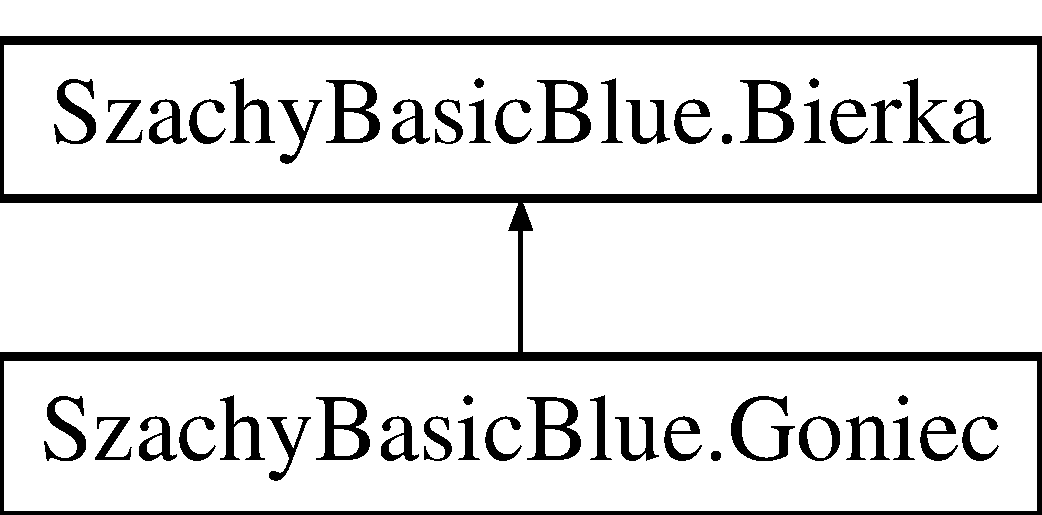
\includegraphics[height=2.000000cm]{class_szachy_basic_blue_1_1_goniec}
\end{center}
\end{figure}
\subsection*{Dodatkowe Dziedziczone Składowe}


\subsection{Opis szczegółowy}


Definicja w linii 3 pliku Goniec.\-cs.



Dokumentacja dla tej klasy została wygenerowana z pliku\-:\begin{DoxyCompactItemize}
\item 
\hyperlink{_goniec_8cs}{Goniec.\-cs}\end{DoxyCompactItemize}

\hypertarget{class_szachy_basic_blue_1_1_gra}{\section{Dokumentacja klasy Szachy\-Basic\-Blue.\-Gra}
\label{class_szachy_basic_blue_1_1_gra}\index{Szachy\-Basic\-Blue.\-Gra@{Szachy\-Basic\-Blue.\-Gra}}
}
Diagram dziedziczenia dla Szachy\-Basic\-Blue.\-Gra\begin{figure}[H]
\begin{center}
\leavevmode
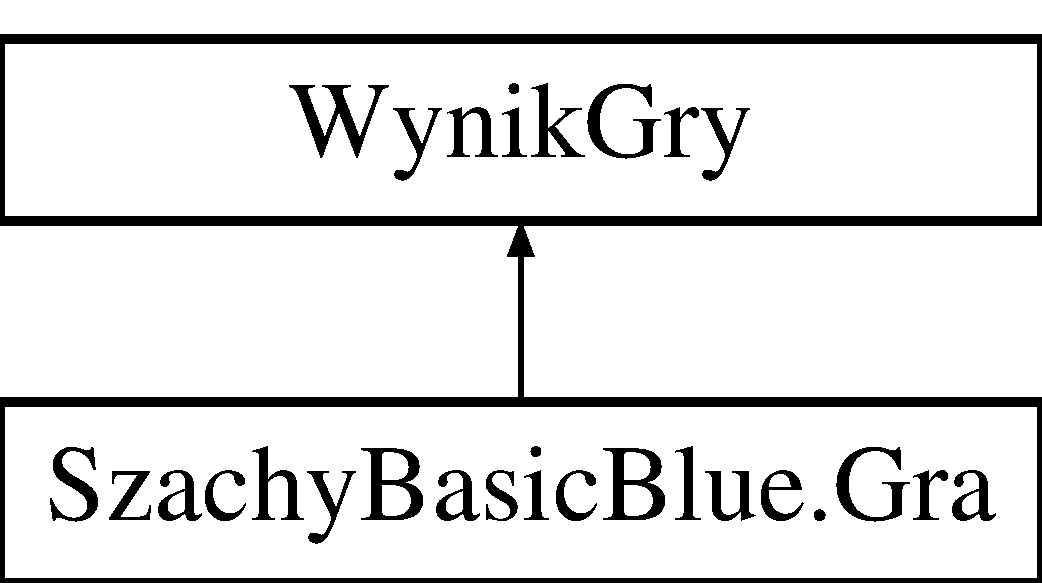
\includegraphics[height=2.000000cm]{class_szachy_basic_blue_1_1_gra}
\end{center}
\end{figure}
\subsection*{Metody publiczne}
\begin{DoxyCompactItemize}
\item 
void \hyperlink{class_szachy_basic_blue_1_1_gra_a5c8dab8fc89c02678a0aec3fc3bc3ff8}{Dodaj\-\_\-\-Ruch} ()
\item 
void \hyperlink{class_szachy_basic_blue_1_1_gra_a6c36702f196d44ecbc4f0a33d26f2759}{Zako�czona} ()
\item 
void \hyperlink{class_szachy_basic_blue_1_1_gra_ac37f4a8f656c34447dda2db9bd07ccbd}{Jest\-Szach\-Mat} ()
\item 
void \hyperlink{class_szachy_basic_blue_1_1_gra_a6472434c00ad4cd718cebb802b637f91}{Operacje} ()
\item 
void \hyperlink{class_szachy_basic_blue_1_1_gra_a2a009688dd9c7b17f5ad13f9a89c5839}{Jest\-\_\-\-Pat} ()
\item 
void \hyperlink{class_szachy_basic_blue_1_1_gra_a009ac8530fd1fc3ddacb3e1505821b5e}{Jest\-\_\-\-Szach} ()
\end{DoxyCompactItemize}
\subsection*{Atrybuty publiczne}
\begin{DoxyCompactItemize}
\item 
string \hyperlink{class_szachy_basic_blue_1_1_gra_a02d48b9af3ccc90cc970f29f7f30693a}{Wyniki}
\item 
string \hyperlink{class_szachy_basic_blue_1_1_gra_a86d2e2c18326bc6451a6ff9f759c4dd5}{Status}
\item 
int \hyperlink{class_szachy_basic_blue_1_1_gra_a1aa54689b6a51e3cebcfe60a83d79551}{Wykonane\-\_\-\-Ruchy}
\item 
\hyperlink{class_szachy_basic_blue_1_1_gracz}{Gracz}\mbox{[}$\,$\mbox{]} \hyperlink{class_szachy_basic_blue_1_1_gra_a28ba407676dbc330d970f5146e765e50}{Gracz}
\begin{DoxyCompactList}\small\item\em Nazwa gracza \end{DoxyCompactList}\item 
bool \hyperlink{class_szachy_basic_blue_1_1_gra_a5853b31e7357153e7a51dd8cf1cb6c49}{Zapis}
\item 
bool \hyperlink{class_szachy_basic_blue_1_1_gra_a83bcb29d76fe2f664664cfde4c41cb8e}{Odczyt}
\end{DoxyCompactItemize}
\subsection*{Atrybuty prywatne}
\begin{DoxyCompactItemize}
\item 
\hyperlink{class_szachy_basic_blue_1_1_historia___ruch_xF3w}{Historia\-\_\-\-Ruch�w} historia \hyperlink{class_szachy_basic_blue_1_1_gra_a63b5d150069f98c615d311b7b496c27e}{Ruch�w}
\item 
\hyperlink{class_szachy_basic_blue_1_1_zapis_gry}{Zapis\-Gry} \hyperlink{class_szachy_basic_blue_1_1_gra_a9e2291aa0d3fe890f27159fa35a65ca3}{zapis\-Gry}
\item 
\hyperlink{class_szachy_basic_blue_1_1_odczyt_gry}{Odczyt\-Gry} \hyperlink{class_szachy_basic_blue_1_1_gra_a95574d607a0c560a4eee747276307a09}{odczyt\-Gry}
\item 
\hyperlink{class_szachy_basic_blue_1_1_gracz}{Gracz} \hyperlink{class_szachy_basic_blue_1_1_gra_a333d0fc461c21a98e1e697208bc03e2b}{gracz}
\item 
\hyperlink{class_szachy_basic_blue_1_1_bierka}{Bierka} \hyperlink{class_szachy_basic_blue_1_1_gra_a677214ff7dc037138c8e1206e5ad6b9e}{bierka}
\end{DoxyCompactItemize}


\subsection{Opis szczegółowy}


Definicja w linii 3 pliku Gra.\-cs.



\subsection{Dokumentacja funkcji składowych}
\hypertarget{class_szachy_basic_blue_1_1_gra_a5c8dab8fc89c02678a0aec3fc3bc3ff8}{\index{Szachy\-Basic\-Blue\-::\-Gra@{Szachy\-Basic\-Blue\-::\-Gra}!Dodaj\-\_\-\-Ruch@{Dodaj\-\_\-\-Ruch}}
\index{Dodaj\-\_\-\-Ruch@{Dodaj\-\_\-\-Ruch}!SzachyBasicBlue::Gra@{Szachy\-Basic\-Blue\-::\-Gra}}
\subsubsection[{Dodaj\-\_\-\-Ruch}]{\setlength{\rightskip}{0pt plus 5cm}void Szachy\-Basic\-Blue.\-Gra.\-Dodaj\-\_\-\-Ruch (
\begin{DoxyParamCaption}
{}
\end{DoxyParamCaption}
)}}\label{class_szachy_basic_blue_1_1_gra_a5c8dab8fc89c02678a0aec3fc3bc3ff8}


Definicja w linii 14 pliku Gra.\-cs.

\hypertarget{class_szachy_basic_blue_1_1_gra_a2a009688dd9c7b17f5ad13f9a89c5839}{\index{Szachy\-Basic\-Blue\-::\-Gra@{Szachy\-Basic\-Blue\-::\-Gra}!Jest\-\_\-\-Pat@{Jest\-\_\-\-Pat}}
\index{Jest\-\_\-\-Pat@{Jest\-\_\-\-Pat}!SzachyBasicBlue::Gra@{Szachy\-Basic\-Blue\-::\-Gra}}
\subsubsection[{Jest\-\_\-\-Pat}]{\setlength{\rightskip}{0pt plus 5cm}void Szachy\-Basic\-Blue.\-Gra.\-Jest\-\_\-\-Pat (
\begin{DoxyParamCaption}
{}
\end{DoxyParamCaption}
)}}\label{class_szachy_basic_blue_1_1_gra_a2a009688dd9c7b17f5ad13f9a89c5839}


Definicja w linii 26 pliku Gra.\-cs.

\hypertarget{class_szachy_basic_blue_1_1_gra_a009ac8530fd1fc3ddacb3e1505821b5e}{\index{Szachy\-Basic\-Blue\-::\-Gra@{Szachy\-Basic\-Blue\-::\-Gra}!Jest\-\_\-\-Szach@{Jest\-\_\-\-Szach}}
\index{Jest\-\_\-\-Szach@{Jest\-\_\-\-Szach}!SzachyBasicBlue::Gra@{Szachy\-Basic\-Blue\-::\-Gra}}
\subsubsection[{Jest\-\_\-\-Szach}]{\setlength{\rightskip}{0pt plus 5cm}void Szachy\-Basic\-Blue.\-Gra.\-Jest\-\_\-\-Szach (
\begin{DoxyParamCaption}
{}
\end{DoxyParamCaption}
)}}\label{class_szachy_basic_blue_1_1_gra_a009ac8530fd1fc3ddacb3e1505821b5e}


Definicja w linii 29 pliku Gra.\-cs.

\hypertarget{class_szachy_basic_blue_1_1_gra_ac37f4a8f656c34447dda2db9bd07ccbd}{\index{Szachy\-Basic\-Blue\-::\-Gra@{Szachy\-Basic\-Blue\-::\-Gra}!Jest\-Szach\-Mat@{Jest\-Szach\-Mat}}
\index{Jest\-Szach\-Mat@{Jest\-Szach\-Mat}!SzachyBasicBlue::Gra@{Szachy\-Basic\-Blue\-::\-Gra}}
\subsubsection[{Jest\-Szach\-Mat}]{\setlength{\rightskip}{0pt plus 5cm}void Szachy\-Basic\-Blue.\-Gra.\-Jest\-Szach\-Mat (
\begin{DoxyParamCaption}
{}
\end{DoxyParamCaption}
)}}\label{class_szachy_basic_blue_1_1_gra_ac37f4a8f656c34447dda2db9bd07ccbd}


Definicja w linii 20 pliku Gra.\-cs.

\hypertarget{class_szachy_basic_blue_1_1_gra_a6472434c00ad4cd718cebb802b637f91}{\index{Szachy\-Basic\-Blue\-::\-Gra@{Szachy\-Basic\-Blue\-::\-Gra}!Operacje@{Operacje}}
\index{Operacje@{Operacje}!SzachyBasicBlue::Gra@{Szachy\-Basic\-Blue\-::\-Gra}}
\subsubsection[{Operacje}]{\setlength{\rightskip}{0pt plus 5cm}void Szachy\-Basic\-Blue.\-Gra.\-Operacje (
\begin{DoxyParamCaption}
{}
\end{DoxyParamCaption}
)}}\label{class_szachy_basic_blue_1_1_gra_a6472434c00ad4cd718cebb802b637f91}


Definicja w linii 23 pliku Gra.\-cs.

\hypertarget{class_szachy_basic_blue_1_1_gra_a6c36702f196d44ecbc4f0a33d26f2759}{\index{Szachy\-Basic\-Blue\-::\-Gra@{Szachy\-Basic\-Blue\-::\-Gra}!Zako�czona@{Zako�czona}}
\index{Zako�czona@{Zako�czona}!SzachyBasicBlue::Gra@{Szachy\-Basic\-Blue\-::\-Gra}}
\subsubsection[{Zako�czona}]{\setlength{\rightskip}{0pt plus 5cm}void Szachy\-Basic\-Blue.\-Gra.\-Zako�czona (
\begin{DoxyParamCaption}
{}
\end{DoxyParamCaption}
)}}\label{class_szachy_basic_blue_1_1_gra_a6c36702f196d44ecbc4f0a33d26f2759}


Definicja w linii 17 pliku Gra.\-cs.



\subsection{Dokumentacja atrybutów składowych}
\hypertarget{class_szachy_basic_blue_1_1_gra_a677214ff7dc037138c8e1206e5ad6b9e}{\index{Szachy\-Basic\-Blue\-::\-Gra@{Szachy\-Basic\-Blue\-::\-Gra}!bierka@{bierka}}
\index{bierka@{bierka}!SzachyBasicBlue::Gra@{Szachy\-Basic\-Blue\-::\-Gra}}
\subsubsection[{bierka}]{\setlength{\rightskip}{0pt plus 5cm}{\bf Bierka} Szachy\-Basic\-Blue.\-Gra.\-bierka\hspace{0.3cm}{\ttfamily [private]}}}\label{class_szachy_basic_blue_1_1_gra_a677214ff7dc037138c8e1206e5ad6b9e}


Definicja w linii 38 pliku Gra.\-cs.

\hypertarget{class_szachy_basic_blue_1_1_gra_a28ba407676dbc330d970f5146e765e50}{\index{Szachy\-Basic\-Blue\-::\-Gra@{Szachy\-Basic\-Blue\-::\-Gra}!Gracz@{Gracz}}
\index{Gracz@{Gracz}!SzachyBasicBlue::Gra@{Szachy\-Basic\-Blue\-::\-Gra}}
\subsubsection[{Gracz}]{\setlength{\rightskip}{0pt plus 5cm}{\bf Gracz} \mbox{[}$\,$\mbox{]} Szachy\-Basic\-Blue.\-Gra.\-Gracz}}\label{class_szachy_basic_blue_1_1_gra_a28ba407676dbc330d970f5146e765e50}


Nazwa gracza 



Definicja w linii 10 pliku Gra.\-cs.

\hypertarget{class_szachy_basic_blue_1_1_gra_a333d0fc461c21a98e1e697208bc03e2b}{\index{Szachy\-Basic\-Blue\-::\-Gra@{Szachy\-Basic\-Blue\-::\-Gra}!gracz@{gracz}}
\index{gracz@{gracz}!SzachyBasicBlue::Gra@{Szachy\-Basic\-Blue\-::\-Gra}}
\subsubsection[{gracz}]{\setlength{\rightskip}{0pt plus 5cm}{\bf Gracz} Szachy\-Basic\-Blue.\-Gra.\-gracz\hspace{0.3cm}{\ttfamily [private]}}}\label{class_szachy_basic_blue_1_1_gra_a333d0fc461c21a98e1e697208bc03e2b}


Definicja w linii 36 pliku Gra.\-cs.

\hypertarget{class_szachy_basic_blue_1_1_gra_a83bcb29d76fe2f664664cfde4c41cb8e}{\index{Szachy\-Basic\-Blue\-::\-Gra@{Szachy\-Basic\-Blue\-::\-Gra}!Odczyt@{Odczyt}}
\index{Odczyt@{Odczyt}!SzachyBasicBlue::Gra@{Szachy\-Basic\-Blue\-::\-Gra}}
\subsubsection[{Odczyt}]{\setlength{\rightskip}{0pt plus 5cm}bool Szachy\-Basic\-Blue.\-Gra.\-Odczyt}}\label{class_szachy_basic_blue_1_1_gra_a83bcb29d76fe2f664664cfde4c41cb8e}


Definicja w linii 12 pliku Gra.\-cs.

\hypertarget{class_szachy_basic_blue_1_1_gra_a95574d607a0c560a4eee747276307a09}{\index{Szachy\-Basic\-Blue\-::\-Gra@{Szachy\-Basic\-Blue\-::\-Gra}!odczyt\-Gry@{odczyt\-Gry}}
\index{odczyt\-Gry@{odczyt\-Gry}!SzachyBasicBlue::Gra@{Szachy\-Basic\-Blue\-::\-Gra}}
\subsubsection[{odczyt\-Gry}]{\setlength{\rightskip}{0pt plus 5cm}{\bf Odczyt\-Gry} Szachy\-Basic\-Blue.\-Gra.\-odczyt\-Gry\hspace{0.3cm}{\ttfamily [private]}}}\label{class_szachy_basic_blue_1_1_gra_a95574d607a0c560a4eee747276307a09}


Definicja w linii 35 pliku Gra.\-cs.

\hypertarget{class_szachy_basic_blue_1_1_gra_a63b5d150069f98c615d311b7b496c27e}{\index{Szachy\-Basic\-Blue\-::\-Gra@{Szachy\-Basic\-Blue\-::\-Gra}!Ruch�w@{Ruch�w}}
\index{Ruch�w@{Ruch�w}!SzachyBasicBlue::Gra@{Szachy\-Basic\-Blue\-::\-Gra}}
\subsubsection[{Ruch�w}]{\setlength{\rightskip}{0pt plus 5cm}{\bf Historia\-\_\-\-Ruch�w} historia Szachy\-Basic\-Blue.\-Gra.\-Ruch�w\hspace{0.3cm}{\ttfamily [private]}}}\label{class_szachy_basic_blue_1_1_gra_a63b5d150069f98c615d311b7b496c27e}


Definicja w linii 33 pliku Gra.\-cs.

\hypertarget{class_szachy_basic_blue_1_1_gra_a86d2e2c18326bc6451a6ff9f759c4dd5}{\index{Szachy\-Basic\-Blue\-::\-Gra@{Szachy\-Basic\-Blue\-::\-Gra}!Status@{Status}}
\index{Status@{Status}!SzachyBasicBlue::Gra@{Szachy\-Basic\-Blue\-::\-Gra}}
\subsubsection[{Status}]{\setlength{\rightskip}{0pt plus 5cm}string Szachy\-Basic\-Blue.\-Gra.\-Status}}\label{class_szachy_basic_blue_1_1_gra_a86d2e2c18326bc6451a6ff9f759c4dd5}


Definicja w linii 5 pliku Gra.\-cs.

\hypertarget{class_szachy_basic_blue_1_1_gra_a1aa54689b6a51e3cebcfe60a83d79551}{\index{Szachy\-Basic\-Blue\-::\-Gra@{Szachy\-Basic\-Blue\-::\-Gra}!Wykonane\-\_\-\-Ruchy@{Wykonane\-\_\-\-Ruchy}}
\index{Wykonane\-\_\-\-Ruchy@{Wykonane\-\_\-\-Ruchy}!SzachyBasicBlue::Gra@{Szachy\-Basic\-Blue\-::\-Gra}}
\subsubsection[{Wykonane\-\_\-\-Ruchy}]{\setlength{\rightskip}{0pt plus 5cm}int Szachy\-Basic\-Blue.\-Gra.\-Wykonane\-\_\-\-Ruchy}}\label{class_szachy_basic_blue_1_1_gra_a1aa54689b6a51e3cebcfe60a83d79551}


Definicja w linii 6 pliku Gra.\-cs.

\hypertarget{class_szachy_basic_blue_1_1_gra_a02d48b9af3ccc90cc970f29f7f30693a}{\index{Szachy\-Basic\-Blue\-::\-Gra@{Szachy\-Basic\-Blue\-::\-Gra}!Wyniki@{Wyniki}}
\index{Wyniki@{Wyniki}!SzachyBasicBlue::Gra@{Szachy\-Basic\-Blue\-::\-Gra}}
\subsubsection[{Wyniki}]{\setlength{\rightskip}{0pt plus 5cm}string Szachy\-Basic\-Blue.\-Gra.\-Wyniki}}\label{class_szachy_basic_blue_1_1_gra_a02d48b9af3ccc90cc970f29f7f30693a}


Definicja w linii 4 pliku Gra.\-cs.

\hypertarget{class_szachy_basic_blue_1_1_gra_a5853b31e7357153e7a51dd8cf1cb6c49}{\index{Szachy\-Basic\-Blue\-::\-Gra@{Szachy\-Basic\-Blue\-::\-Gra}!Zapis@{Zapis}}
\index{Zapis@{Zapis}!SzachyBasicBlue::Gra@{Szachy\-Basic\-Blue\-::\-Gra}}
\subsubsection[{Zapis}]{\setlength{\rightskip}{0pt plus 5cm}bool Szachy\-Basic\-Blue.\-Gra.\-Zapis}}\label{class_szachy_basic_blue_1_1_gra_a5853b31e7357153e7a51dd8cf1cb6c49}


Definicja w linii 11 pliku Gra.\-cs.

\hypertarget{class_szachy_basic_blue_1_1_gra_a9e2291aa0d3fe890f27159fa35a65ca3}{\index{Szachy\-Basic\-Blue\-::\-Gra@{Szachy\-Basic\-Blue\-::\-Gra}!zapis\-Gry@{zapis\-Gry}}
\index{zapis\-Gry@{zapis\-Gry}!SzachyBasicBlue::Gra@{Szachy\-Basic\-Blue\-::\-Gra}}
\subsubsection[{zapis\-Gry}]{\setlength{\rightskip}{0pt plus 5cm}{\bf Zapis\-Gry} Szachy\-Basic\-Blue.\-Gra.\-zapis\-Gry\hspace{0.3cm}{\ttfamily [private]}}}\label{class_szachy_basic_blue_1_1_gra_a9e2291aa0d3fe890f27159fa35a65ca3}


Definicja w linii 34 pliku Gra.\-cs.



Dokumentacja dla tej klasy została wygenerowana z pliku\-:\begin{DoxyCompactItemize}
\item 
\hyperlink{_gra_8cs}{Gra.\-cs}\end{DoxyCompactItemize}

\hypertarget{class_szachy_basic_blue_1_1_gracz}{\section{Dokumentacja klasy Szachy\-Basic\-Blue.\-Gracz}
\label{class_szachy_basic_blue_1_1_gracz}\index{Szachy\-Basic\-Blue.\-Gracz@{Szachy\-Basic\-Blue.\-Gracz}}
}
Diagram dziedziczenia dla Szachy\-Basic\-Blue.\-Gracz\begin{figure}[H]
\begin{center}
\leavevmode
\includegraphics[height=2.000000cm]{class_szachy_basic_blue_1_1_gracz}
\end{center}
\end{figure}
\subsection*{Atrybuty publiczne}
\begin{DoxyCompactItemize}
\item 
\hyperlink{namespace_szachy_basic_blue_a247cb874e8c4304fa09e07a257a78277}{Kolor\-\_\-\-Gracza} \hyperlink{class_szachy_basic_blue_1_1_gracz_a1ead8290dd8833563a97ab2a9ee47f7c}{Kolor\-Gracza}
\item 
String \hyperlink{class_szachy_basic_blue_1_1_gracz_a197b73341a7fd21ebe1f036f12c02bd3}{zrob\-Ruch}
\end{DoxyCompactItemize}
\subsection*{Atrybuty prywatne}
\begin{DoxyCompactItemize}
\item 
String \hyperlink{class_szachy_basic_blue_1_1_gracz_ad8698b29d6554cefa6143fb2d8b69451}{silnik\-Gracza}
\item 
\hyperlink{class_szachy_basic_blue_1_1_gra}{Gra} \hyperlink{class_szachy_basic_blue_1_1_gracz_a87917de01bff4f9a56543f05b95bd4d3}{gra}
\end{DoxyCompactItemize}


\subsection{Opis szczegółowy}


Definicja w linii 3 pliku Gracz.\-cs.



\subsection{Dokumentacja atrybutów składowych}
\hypertarget{class_szachy_basic_blue_1_1_gracz_a87917de01bff4f9a56543f05b95bd4d3}{\index{Szachy\-Basic\-Blue\-::\-Gracz@{Szachy\-Basic\-Blue\-::\-Gracz}!gra@{gra}}
\index{gra@{gra}!SzachyBasicBlue::Gracz@{Szachy\-Basic\-Blue\-::\-Gracz}}
\subsubsection[{gra}]{\setlength{\rightskip}{0pt plus 5cm}{\bf Gra} Szachy\-Basic\-Blue.\-Gracz.\-gra\hspace{0.3cm}{\ttfamily [private]}}}\label{class_szachy_basic_blue_1_1_gracz_a87917de01bff4f9a56543f05b95bd4d3}


Definicja w linii 8 pliku Gracz.\-cs.

\hypertarget{class_szachy_basic_blue_1_1_gracz_a1ead8290dd8833563a97ab2a9ee47f7c}{\index{Szachy\-Basic\-Blue\-::\-Gracz@{Szachy\-Basic\-Blue\-::\-Gracz}!Kolor\-Gracza@{Kolor\-Gracza}}
\index{Kolor\-Gracza@{Kolor\-Gracza}!SzachyBasicBlue::Gracz@{Szachy\-Basic\-Blue\-::\-Gracz}}
\subsubsection[{Kolor\-Gracza}]{\setlength{\rightskip}{0pt plus 5cm}{\bf Kolor\-\_\-\-Gracza} Szachy\-Basic\-Blue.\-Gracz.\-Kolor\-Gracza}}\label{class_szachy_basic_blue_1_1_gracz_a1ead8290dd8833563a97ab2a9ee47f7c}


Definicja w linii 4 pliku Gracz.\-cs.

\hypertarget{class_szachy_basic_blue_1_1_gracz_ad8698b29d6554cefa6143fb2d8b69451}{\index{Szachy\-Basic\-Blue\-::\-Gracz@{Szachy\-Basic\-Blue\-::\-Gracz}!silnik\-Gracza@{silnik\-Gracza}}
\index{silnik\-Gracza@{silnik\-Gracza}!SzachyBasicBlue::Gracz@{Szachy\-Basic\-Blue\-::\-Gracz}}
\subsubsection[{silnik\-Gracza}]{\setlength{\rightskip}{0pt plus 5cm}String Szachy\-Basic\-Blue.\-Gracz.\-silnik\-Gracza\hspace{0.3cm}{\ttfamily [private]}}}\label{class_szachy_basic_blue_1_1_gracz_ad8698b29d6554cefa6143fb2d8b69451}


Definicja w linii 5 pliku Gracz.\-cs.

\hypertarget{class_szachy_basic_blue_1_1_gracz_a197b73341a7fd21ebe1f036f12c02bd3}{\index{Szachy\-Basic\-Blue\-::\-Gracz@{Szachy\-Basic\-Blue\-::\-Gracz}!zrob\-Ruch@{zrob\-Ruch}}
\index{zrob\-Ruch@{zrob\-Ruch}!SzachyBasicBlue::Gracz@{Szachy\-Basic\-Blue\-::\-Gracz}}
\subsubsection[{zrob\-Ruch}]{\setlength{\rightskip}{0pt plus 5cm}String Szachy\-Basic\-Blue.\-Gracz.\-zrob\-Ruch}}\label{class_szachy_basic_blue_1_1_gracz_a197b73341a7fd21ebe1f036f12c02bd3}


Definicja w linii 6 pliku Gracz.\-cs.



Dokumentacja dla tej klasy została wygenerowana z pliku\-:\begin{DoxyCompactItemize}
\item 
\hyperlink{_gracz_8cs}{Gracz.\-cs}\end{DoxyCompactItemize}

\hypertarget{class_szachy_basic_blue_1_1_hetman}{\section{Dokumentacja klasy Szachy\-Basic\-Blue.\-Hetman}
\label{class_szachy_basic_blue_1_1_hetman}\index{Szachy\-Basic\-Blue.\-Hetman@{Szachy\-Basic\-Blue.\-Hetman}}
}
Diagram dziedziczenia dla Szachy\-Basic\-Blue.\-Hetman\begin{figure}[H]
\begin{center}
\leavevmode
\includegraphics[height=2.000000cm]{class_szachy_basic_blue_1_1_hetman}
\end{center}
\end{figure}
\subsection*{Dodatkowe Dziedziczone Składowe}


\subsection{Opis szczegółowy}


Definicja w linii 3 pliku Hetman.\-cs.



Dokumentacja dla tej klasy została wygenerowana z pliku\-:\begin{DoxyCompactItemize}
\item 
\hyperlink{_hetman_8cs}{Hetman.\-cs}\end{DoxyCompactItemize}

\hypertarget{class_szachy_basic_blue_1_1_historia___ruch_xF3w}{\section{Dokumentacja klasy Szachy\-Basic\-Blue.\-Historia\-\_\-\-Ruch�w}
\label{class_szachy_basic_blue_1_1_historia___ruch_xF3w}\index{Szachy\-Basic\-Blue.\-Historia\-\_\-\-Ruch�w@{Szachy\-Basic\-Blue.\-Historia\-\_\-\-Ruch�w}}
}
\subsection*{Metody publiczne}
\begin{DoxyCompactItemize}
\item 
void \hyperlink{class_szachy_basic_blue_1_1_historia___ruch_xF3w_a7304bdf73e221ff1748726c1856f44ac}{Notacja\-\_\-algebraiczna} ()
\end{DoxyCompactItemize}
\subsection*{Atrybuty prywatne}
\begin{DoxyCompactItemize}
\item 
\hyperlink{class_szachy_basic_blue_1_1_gra}{Gra} \hyperlink{class_szachy_basic_blue_1_1_historia___ruch_xF3w_a2687123081558893b3d3258ed36acfdc}{gra}
\end{DoxyCompactItemize}


\subsection{Opis szczegółowy}


Definicja w linii 3 pliku Historia\-\_\-\-Ruchów.\-cs.



\subsection{Dokumentacja funkcji składowych}
\hypertarget{class_szachy_basic_blue_1_1_historia___ruch_xF3w_a7304bdf73e221ff1748726c1856f44ac}{\index{Szachy\-Basic\-Blue\-::\-Historia\-\_\-\-Ruch�w@{Szachy\-Basic\-Blue\-::\-Historia\-\_\-\-Ruch�w}!Notacja\-\_\-algebraiczna@{Notacja\-\_\-algebraiczna}}
\index{Notacja\-\_\-algebraiczna@{Notacja\-\_\-algebraiczna}!SzachyBasicBlue::Historia_Ruch�w@{Szachy\-Basic\-Blue\-::\-Historia\-\_\-\-Ruch�w}}
\subsubsection[{Notacja\-\_\-algebraiczna}]{\setlength{\rightskip}{0pt plus 5cm}void Szachy\-Basic\-Blue.\-Historia\-\_\-\-Ruch�w.\-Notacja\-\_\-algebraiczna (
\begin{DoxyParamCaption}
{}
\end{DoxyParamCaption}
)}}\label{class_szachy_basic_blue_1_1_historia___ruch_xF3w_a7304bdf73e221ff1748726c1856f44ac}


Definicja w linii 4 pliku Historia\-\_\-\-Ruchów.\-cs.



\subsection{Dokumentacja atrybutów składowych}
\hypertarget{class_szachy_basic_blue_1_1_historia___ruch_xF3w_a2687123081558893b3d3258ed36acfdc}{\index{Szachy\-Basic\-Blue\-::\-Historia\-\_\-\-Ruch�w@{Szachy\-Basic\-Blue\-::\-Historia\-\_\-\-Ruch�w}!gra@{gra}}
\index{gra@{gra}!SzachyBasicBlue::Historia_Ruch�w@{Szachy\-Basic\-Blue\-::\-Historia\-\_\-\-Ruch�w}}
\subsubsection[{gra}]{\setlength{\rightskip}{0pt plus 5cm}{\bf Gra} Szachy\-Basic\-Blue.\-Historia\-\_\-\-Ruch�w.\-gra\hspace{0.3cm}{\ttfamily [private]}}}\label{class_szachy_basic_blue_1_1_historia___ruch_xF3w_a2687123081558893b3d3258ed36acfdc}


Definicja w linii 8 pliku Historia\-\_\-\-Ruchów.\-cs.



Dokumentacja dla tej klasy została wygenerowana z pliku\-:\begin{DoxyCompactItemize}
\item 
\hyperlink{_historia___ruch_xC3_xB3w_8cs}{Historia\-\_\-\-Ruchów.\-cs}\end{DoxyCompactItemize}

\hypertarget{class_szachy_basic_blue_1_1_komputer}{\section{Dokumentacja klasy Szachy\-Basic\-Blue.\-Komputer}
\label{class_szachy_basic_blue_1_1_komputer}\index{Szachy\-Basic\-Blue.\-Komputer@{Szachy\-Basic\-Blue.\-Komputer}}
}
Diagram dziedziczenia dla Szachy\-Basic\-Blue.\-Komputer\begin{figure}[H]
\begin{center}
\leavevmode
\includegraphics[height=2.000000cm]{class_szachy_basic_blue_1_1_komputer}
\end{center}
\end{figure}
\subsection*{Metody publiczne}
\begin{DoxyCompactItemize}
\item 
void \hyperlink{class_szachy_basic_blue_1_1_komputer_a495dfb194e8c46422ddea7739176ecce}{Zr�b\-\_\-\-Ruch} ()
\end{DoxyCompactItemize}
\subsection*{Atrybuty publiczne}
\begin{DoxyCompactItemize}
\item 
String \hyperlink{class_szachy_basic_blue_1_1_komputer_a570a60111ddd10a7918d55ba75bf5671}{zrob\-Ruch}
\end{DoxyCompactItemize}


\subsection{Opis szczegółowy}


Definicja w linii 3 pliku Gracz-\/\-Komputer.\-cs.



\subsection{Dokumentacja funkcji składowych}
\hypertarget{class_szachy_basic_blue_1_1_komputer_a495dfb194e8c46422ddea7739176ecce}{\index{Szachy\-Basic\-Blue\-::\-Komputer@{Szachy\-Basic\-Blue\-::\-Komputer}!Zr�b\-\_\-\-Ruch@{Zr�b\-\_\-\-Ruch}}
\index{Zr�b\-\_\-\-Ruch@{Zr�b\-\_\-\-Ruch}!SzachyBasicBlue::Komputer@{Szachy\-Basic\-Blue\-::\-Komputer}}
\subsubsection[{Zr�b\-\_\-\-Ruch}]{\setlength{\rightskip}{0pt plus 5cm}void Szachy\-Basic\-Blue.\-Komputer.\-Zr�b\-\_\-\-Ruch (
\begin{DoxyParamCaption}
{}
\end{DoxyParamCaption}
)}}\label{class_szachy_basic_blue_1_1_komputer_a495dfb194e8c46422ddea7739176ecce}


Definicja w linii 6 pliku Gracz-\/\-Komputer.\-cs.



\subsection{Dokumentacja atrybutów składowych}
\hypertarget{class_szachy_basic_blue_1_1_komputer_a570a60111ddd10a7918d55ba75bf5671}{\index{Szachy\-Basic\-Blue\-::\-Komputer@{Szachy\-Basic\-Blue\-::\-Komputer}!zrob\-Ruch@{zrob\-Ruch}}
\index{zrob\-Ruch@{zrob\-Ruch}!SzachyBasicBlue::Komputer@{Szachy\-Basic\-Blue\-::\-Komputer}}
\subsubsection[{zrob\-Ruch}]{\setlength{\rightskip}{0pt plus 5cm}String Szachy\-Basic\-Blue.\-Komputer.\-zrob\-Ruch}}\label{class_szachy_basic_blue_1_1_komputer_a570a60111ddd10a7918d55ba75bf5671}


Definicja w linii 4 pliku Gracz-\/\-Komputer.\-cs.



Dokumentacja dla tej klasy została wygenerowana z pliku\-:\begin{DoxyCompactItemize}
\item 
\hyperlink{_gracz-_komputer_8cs}{Gracz-\/\-Komputer.\-cs}\end{DoxyCompactItemize}

\hypertarget{class_szachy_basic_blue_1_1_kr_xF3l}{\section{Dokumentacja klasy Szachy\-Basic\-Blue.\-Kr�l}
\label{class_szachy_basic_blue_1_1_kr_xF3l}\index{Szachy\-Basic\-Blue.\-Kr�l@{Szachy\-Basic\-Blue.\-Kr�l}}
}
Diagram dziedziczenia dla Szachy\-Basic\-Blue.\-Kr�l\begin{figure}[H]
\begin{center}
\leavevmode
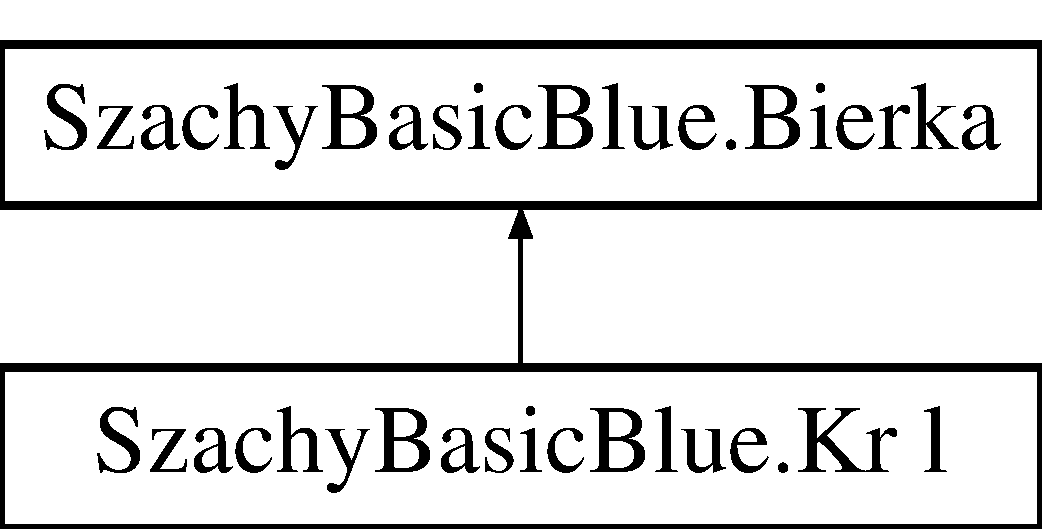
\includegraphics[height=2.000000cm]{class_szachy_basic_blue_1_1_kr_xF3l}
\end{center}
\end{figure}
\subsection*{Dodatkowe Dziedziczone Składowe}


\subsection{Opis szczegółowy}


Definicja w linii 3 pliku Król.\-cs.



Dokumentacja dla tej klasy została wygenerowana z pliku\-:\begin{DoxyCompactItemize}
\item 
\hyperlink{_kr_xC3_xB3l_8cs}{Król.\-cs}\end{DoxyCompactItemize}

\hypertarget{class_szachy_basic_blue_1_1_odczyt_gry}{\section{Dokumentacja klasy Szachy\-Basic\-Blue.\-Odczyt\-Gry}
\label{class_szachy_basic_blue_1_1_odczyt_gry}\index{Szachy\-Basic\-Blue.\-Odczyt\-Gry@{Szachy\-Basic\-Blue.\-Odczyt\-Gry}}
}
\subsection*{Metody publiczne}
\begin{DoxyCompactItemize}
\item 
void \hyperlink{class_szachy_basic_blue_1_1_odczyt_gry_ac633213082d31e39de17dcf431ed679b}{Open} ()
\end{DoxyCompactItemize}
\subsection*{Atrybuty prywatne}
\begin{DoxyCompactItemize}
\item 
\hyperlink{class_szachy_basic_blue_1_1_gra}{Gra} \hyperlink{class_szachy_basic_blue_1_1_odczyt_gry_aa31f0e6621c5259169ccd0cb12ae74e1}{gra}
\end{DoxyCompactItemize}


\subsection{Opis szczegółowy}


Definicja w linii 3 pliku Odczyt\-Gry.\-cs.



\subsection{Dokumentacja funkcji składowych}
\hypertarget{class_szachy_basic_blue_1_1_odczyt_gry_ac633213082d31e39de17dcf431ed679b}{\index{Szachy\-Basic\-Blue\-::\-Odczyt\-Gry@{Szachy\-Basic\-Blue\-::\-Odczyt\-Gry}!Open@{Open}}
\index{Open@{Open}!SzachyBasicBlue::OdczytGry@{Szachy\-Basic\-Blue\-::\-Odczyt\-Gry}}
\subsubsection[{Open}]{\setlength{\rightskip}{0pt plus 5cm}void Szachy\-Basic\-Blue.\-Odczyt\-Gry.\-Open (
\begin{DoxyParamCaption}
{}
\end{DoxyParamCaption}
)}}\label{class_szachy_basic_blue_1_1_odczyt_gry_ac633213082d31e39de17dcf431ed679b}


Definicja w linii 4 pliku Odczyt\-Gry.\-cs.



\subsection{Dokumentacja atrybutów składowych}
\hypertarget{class_szachy_basic_blue_1_1_odczyt_gry_aa31f0e6621c5259169ccd0cb12ae74e1}{\index{Szachy\-Basic\-Blue\-::\-Odczyt\-Gry@{Szachy\-Basic\-Blue\-::\-Odczyt\-Gry}!gra@{gra}}
\index{gra@{gra}!SzachyBasicBlue::OdczytGry@{Szachy\-Basic\-Blue\-::\-Odczyt\-Gry}}
\subsubsection[{gra}]{\setlength{\rightskip}{0pt plus 5cm}{\bf Gra} Szachy\-Basic\-Blue.\-Odczyt\-Gry.\-gra\hspace{0.3cm}{\ttfamily [private]}}}\label{class_szachy_basic_blue_1_1_odczyt_gry_aa31f0e6621c5259169ccd0cb12ae74e1}


Definicja w linii 8 pliku Odczyt\-Gry.\-cs.



Dokumentacja dla tej klasy została wygenerowana z pliku\-:\begin{DoxyCompactItemize}
\item 
\hyperlink{_odczyt_gry_8cs}{Odczyt\-Gry.\-cs}\end{DoxyCompactItemize}

\hypertarget{class_szachy_basic_blue_1_1_pionek}{\section{Dokumentacja klasy Szachy\-Basic\-Blue.\-Pionek}
\label{class_szachy_basic_blue_1_1_pionek}\index{Szachy\-Basic\-Blue.\-Pionek@{Szachy\-Basic\-Blue.\-Pionek}}
}
Diagram dziedziczenia dla Szachy\-Basic\-Blue.\-Pionek\begin{figure}[H]
\begin{center}
\leavevmode
\includegraphics[height=2.000000cm]{class_szachy_basic_blue_1_1_pionek}
\end{center}
\end{figure}
\subsection*{Atrybuty publiczne}
\begin{DoxyCompactItemize}
\item 
\hyperlink{namespace_szachy_basic_blue_aa6e0b1a326ce3bc4ad1c8737343f55dc}{Kierunek\-Ruchu} \hyperlink{class_szachy_basic_blue_1_1_pionek_a9ad7471a3a1b9e69cdfabaeea8e7327d}{Kierunek\-\_\-\-Ruchu}
\begin{DoxyCompactList}\small\item\em \hyperlink{class_szachy_basic_blue_1_1_pionek}{Pionek} mo�e porusza� si� tylko do przodu, a bij�c na skos \end{DoxyCompactList}\end{DoxyCompactItemize}
\subsection*{Atrybuty prywatne}
\begin{DoxyCompactItemize}
\item 
bool \hyperlink{class_szachy_basic_blue_1_1_pionek_ad1472d4134d04c837e5dff6e7ab7effa}{promocja}
\item 
\hyperlink{class_szachy_basic_blue_1_1_pionki___gracza}{Pionki\-\_\-\-Gracza} \hyperlink{class_szachy_basic_blue_1_1_pionek_ab28d05004bf02b5c11ee988db7b31138}{promocja\-\_\-\-Do}
\end{DoxyCompactItemize}
\subsection*{Dodatkowe Dziedziczone Składowe}


\subsection{Opis szczegółowy}


Definicja w linii 3 pliku Pionek.\-cs.



\subsection{Dokumentacja atrybutów składowych}
\hypertarget{class_szachy_basic_blue_1_1_pionek_a9ad7471a3a1b9e69cdfabaeea8e7327d}{\index{Szachy\-Basic\-Blue\-::\-Pionek@{Szachy\-Basic\-Blue\-::\-Pionek}!Kierunek\-\_\-\-Ruchu@{Kierunek\-\_\-\-Ruchu}}
\index{Kierunek\-\_\-\-Ruchu@{Kierunek\-\_\-\-Ruchu}!SzachyBasicBlue::Pionek@{Szachy\-Basic\-Blue\-::\-Pionek}}
\subsubsection[{Kierunek\-\_\-\-Ruchu}]{\setlength{\rightskip}{0pt plus 5cm}{\bf Kierunek\-Ruchu} Szachy\-Basic\-Blue.\-Pionek.\-Kierunek\-\_\-\-Ruchu}}\label{class_szachy_basic_blue_1_1_pionek_a9ad7471a3a1b9e69cdfabaeea8e7327d}


\hyperlink{class_szachy_basic_blue_1_1_pionek}{Pionek} mo�e porusza� si� tylko do przodu, a bij�c na skos 



Definicja w linii 7 pliku Pionek.\-cs.

\hypertarget{class_szachy_basic_blue_1_1_pionek_ad1472d4134d04c837e5dff6e7ab7effa}{\index{Szachy\-Basic\-Blue\-::\-Pionek@{Szachy\-Basic\-Blue\-::\-Pionek}!promocja@{promocja}}
\index{promocja@{promocja}!SzachyBasicBlue::Pionek@{Szachy\-Basic\-Blue\-::\-Pionek}}
\subsubsection[{promocja}]{\setlength{\rightskip}{0pt plus 5cm}bool Szachy\-Basic\-Blue.\-Pionek.\-promocja\hspace{0.3cm}{\ttfamily [private]}}}\label{class_szachy_basic_blue_1_1_pionek_ad1472d4134d04c837e5dff6e7ab7effa}


Definicja w linii 8 pliku Pionek.\-cs.

\hypertarget{class_szachy_basic_blue_1_1_pionek_ab28d05004bf02b5c11ee988db7b31138}{\index{Szachy\-Basic\-Blue\-::\-Pionek@{Szachy\-Basic\-Blue\-::\-Pionek}!promocja\-\_\-\-Do@{promocja\-\_\-\-Do}}
\index{promocja\-\_\-\-Do@{promocja\-\_\-\-Do}!SzachyBasicBlue::Pionek@{Szachy\-Basic\-Blue\-::\-Pionek}}
\subsubsection[{promocja\-\_\-\-Do}]{\setlength{\rightskip}{0pt plus 5cm}{\bf Pionki\-\_\-\-Gracza} Szachy\-Basic\-Blue.\-Pionek.\-promocja\-\_\-\-Do\hspace{0.3cm}{\ttfamily [private]}}}\label{class_szachy_basic_blue_1_1_pionek_ab28d05004bf02b5c11ee988db7b31138}


Definicja w linii 9 pliku Pionek.\-cs.



Dokumentacja dla tej klasy została wygenerowana z pliku\-:\begin{DoxyCompactItemize}
\item 
\hyperlink{_pionek_8cs}{Pionek.\-cs}\end{DoxyCompactItemize}

\hypertarget{class_szachy_basic_blue_1_1_pionki___gracza}{\section{Dokumentacja klasy Szachy\-Basic\-Blue.\-Pionki\-\_\-\-Gracza}
\label{class_szachy_basic_blue_1_1_pionki___gracza}\index{Szachy\-Basic\-Blue.\-Pionki\-\_\-\-Gracza@{Szachy\-Basic\-Blue.\-Pionki\-\_\-\-Gracza}}
}
\subsection*{Atrybuty publiczne}
\begin{DoxyCompactItemize}
\item 
string \hyperlink{class_szachy_basic_blue_1_1_pionki___gracza_af92a1285e98224184d83bcc77ba69e9f}{Pionki}
\item 
string \hyperlink{class_szachy_basic_blue_1_1_pionki___gracza_af6f6c6b9f0068cedae2da45843fa4a11}{Kolor}
\begin{DoxyCompactList}\small\item\em Kolor Pionka \end{DoxyCompactList}\end{DoxyCompactItemize}
\subsection*{Atrybuty prywatne}
\begin{DoxyCompactItemize}
\item 
\hyperlink{class_szachy_basic_blue_1_1_bierka}{Bierka} \hyperlink{class_szachy_basic_blue_1_1_pionki___gracza_ae84a422688851904d03ae1753bd11771}{bierka}
\item 
\hyperlink{class_szachy_basic_blue_1_1_szachownica}{Szachownica} \hyperlink{class_szachy_basic_blue_1_1_pionki___gracza_aa9823f1f70be577121fa7956e143858d}{szachownica}
\end{DoxyCompactItemize}


\subsection{Opis szczegółowy}


Definicja w linii 3 pliku Pionki\-\_\-\-Gracza.\-cs.



\subsection{Dokumentacja atrybutów składowych}
\hypertarget{class_szachy_basic_blue_1_1_pionki___gracza_ae84a422688851904d03ae1753bd11771}{\index{Szachy\-Basic\-Blue\-::\-Pionki\-\_\-\-Gracza@{Szachy\-Basic\-Blue\-::\-Pionki\-\_\-\-Gracza}!bierka@{bierka}}
\index{bierka@{bierka}!SzachyBasicBlue::Pionki_Gracza@{Szachy\-Basic\-Blue\-::\-Pionki\-\_\-\-Gracza}}
\subsubsection[{bierka}]{\setlength{\rightskip}{0pt plus 5cm}{\bf Bierka} Szachy\-Basic\-Blue.\-Pionki\-\_\-\-Gracza.\-bierka\hspace{0.3cm}{\ttfamily [private]}}}\label{class_szachy_basic_blue_1_1_pionki___gracza_ae84a422688851904d03ae1753bd11771}


Definicja w linii 10 pliku Pionki\-\_\-\-Gracza.\-cs.

\hypertarget{class_szachy_basic_blue_1_1_pionki___gracza_af6f6c6b9f0068cedae2da45843fa4a11}{\index{Szachy\-Basic\-Blue\-::\-Pionki\-\_\-\-Gracza@{Szachy\-Basic\-Blue\-::\-Pionki\-\_\-\-Gracza}!Kolor@{Kolor}}
\index{Kolor@{Kolor}!SzachyBasicBlue::Pionki_Gracza@{Szachy\-Basic\-Blue\-::\-Pionki\-\_\-\-Gracza}}
\subsubsection[{Kolor}]{\setlength{\rightskip}{0pt plus 5cm}string Szachy\-Basic\-Blue.\-Pionki\-\_\-\-Gracza.\-Kolor}}\label{class_szachy_basic_blue_1_1_pionki___gracza_af6f6c6b9f0068cedae2da45843fa4a11}


Kolor Pionka 



Definicja w linii 8 pliku Pionki\-\_\-\-Gracza.\-cs.

\hypertarget{class_szachy_basic_blue_1_1_pionki___gracza_af92a1285e98224184d83bcc77ba69e9f}{\index{Szachy\-Basic\-Blue\-::\-Pionki\-\_\-\-Gracza@{Szachy\-Basic\-Blue\-::\-Pionki\-\_\-\-Gracza}!Pionki@{Pionki}}
\index{Pionki@{Pionki}!SzachyBasicBlue::Pionki_Gracza@{Szachy\-Basic\-Blue\-::\-Pionki\-\_\-\-Gracza}}
\subsubsection[{Pionki}]{\setlength{\rightskip}{0pt plus 5cm}string Szachy\-Basic\-Blue.\-Pionki\-\_\-\-Gracza.\-Pionki}}\label{class_szachy_basic_blue_1_1_pionki___gracza_af92a1285e98224184d83bcc77ba69e9f}


Definicja w linii 4 pliku Pionki\-\_\-\-Gracza.\-cs.

\hypertarget{class_szachy_basic_blue_1_1_pionki___gracza_aa9823f1f70be577121fa7956e143858d}{\index{Szachy\-Basic\-Blue\-::\-Pionki\-\_\-\-Gracza@{Szachy\-Basic\-Blue\-::\-Pionki\-\_\-\-Gracza}!szachownica@{szachownica}}
\index{szachownica@{szachownica}!SzachyBasicBlue::Pionki_Gracza@{Szachy\-Basic\-Blue\-::\-Pionki\-\_\-\-Gracza}}
\subsubsection[{szachownica}]{\setlength{\rightskip}{0pt plus 5cm}{\bf Szachownica} Szachy\-Basic\-Blue.\-Pionki\-\_\-\-Gracza.\-szachownica\hspace{0.3cm}{\ttfamily [private]}}}\label{class_szachy_basic_blue_1_1_pionki___gracza_aa9823f1f70be577121fa7956e143858d}


Definicja w linii 12 pliku Pionki\-\_\-\-Gracza.\-cs.



Dokumentacja dla tej klasy została wygenerowana z pliku\-:\begin{DoxyCompactItemize}
\item 
\hyperlink{_pionki___gracza_8cs}{Pionki\-\_\-\-Gracza.\-cs}\end{DoxyCompactItemize}

\hypertarget{class_szachy_basic_blue_1_1_presti_xBF}{\section{Dokumentacja klasy Szachy\-Basic\-Blue.\-Presti�}
\label{class_szachy_basic_blue_1_1_presti_xBF}\index{Szachy\-Basic\-Blue.\-Presti�@{Szachy\-Basic\-Blue.\-Presti�}}
}


Nadanie presti�u wszystkim figurom  


\subsection*{Atrybuty prywatne}
\begin{DoxyCompactItemize}
\item 
String \hyperlink{class_szachy_basic_blue_1_1_presti_xBF_aafa81d5f88131c2c663e89197f86b53d}{kr�l}
\item 
String \hyperlink{class_szachy_basic_blue_1_1_presti_xBF_aa6803fd91dcba66941f904a6340affcd}{hetman}
\item 
String \hyperlink{class_szachy_basic_blue_1_1_presti_xBF_a57794c98524202b1f1a22d64e7cf73e1}{wie�a}
\item 
String \hyperlink{class_szachy_basic_blue_1_1_presti_xBF_abdffea1a89f82efda86b362ca532b951}{goniec}
\item 
String \hyperlink{class_szachy_basic_blue_1_1_presti_xBF_a57f72c643a526cc8cb8eb37a7afd8d40}{skoczek}
\item 
String \hyperlink{class_szachy_basic_blue_1_1_presti_xBF_a72e5b596af63bac0ed1f5f143299fc05}{pion}
\end{DoxyCompactItemize}


\subsection{Opis szczegółowy}
Nadanie presti�u wszystkim figurom 



Definicja w linii 6 pliku Prestiż.\-cs.



\subsection{Dokumentacja atrybutów składowych}
\hypertarget{class_szachy_basic_blue_1_1_presti_xBF_abdffea1a89f82efda86b362ca532b951}{\index{Szachy\-Basic\-Blue\-::\-Presti�@{Szachy\-Basic\-Blue\-::\-Presti�}!goniec@{goniec}}
\index{goniec@{goniec}!SzachyBasicBlue::Presti�@{Szachy\-Basic\-Blue\-::\-Presti�}}
\subsubsection[{goniec}]{\setlength{\rightskip}{0pt plus 5cm}String Szachy\-Basic\-Blue.\-Presti�.\-goniec\hspace{0.3cm}{\ttfamily [private]}}}\label{class_szachy_basic_blue_1_1_presti_xBF_abdffea1a89f82efda86b362ca532b951}


Definicja w linii 10 pliku Prestiż.\-cs.

\hypertarget{class_szachy_basic_blue_1_1_presti_xBF_aa6803fd91dcba66941f904a6340affcd}{\index{Szachy\-Basic\-Blue\-::\-Presti�@{Szachy\-Basic\-Blue\-::\-Presti�}!hetman@{hetman}}
\index{hetman@{hetman}!SzachyBasicBlue::Presti�@{Szachy\-Basic\-Blue\-::\-Presti�}}
\subsubsection[{hetman}]{\setlength{\rightskip}{0pt plus 5cm}String Szachy\-Basic\-Blue.\-Presti�.\-hetman\hspace{0.3cm}{\ttfamily [private]}}}\label{class_szachy_basic_blue_1_1_presti_xBF_aa6803fd91dcba66941f904a6340affcd}


Definicja w linii 8 pliku Prestiż.\-cs.

\hypertarget{class_szachy_basic_blue_1_1_presti_xBF_aafa81d5f88131c2c663e89197f86b53d}{\index{Szachy\-Basic\-Blue\-::\-Presti�@{Szachy\-Basic\-Blue\-::\-Presti�}!kr�l@{kr�l}}
\index{kr�l@{kr�l}!SzachyBasicBlue::Presti�@{Szachy\-Basic\-Blue\-::\-Presti�}}
\subsubsection[{kr�l}]{\setlength{\rightskip}{0pt plus 5cm}String Szachy\-Basic\-Blue.\-Presti�.\-kr�l\hspace{0.3cm}{\ttfamily [private]}}}\label{class_szachy_basic_blue_1_1_presti_xBF_aafa81d5f88131c2c663e89197f86b53d}


Definicja w linii 7 pliku Prestiż.\-cs.

\hypertarget{class_szachy_basic_blue_1_1_presti_xBF_a72e5b596af63bac0ed1f5f143299fc05}{\index{Szachy\-Basic\-Blue\-::\-Presti�@{Szachy\-Basic\-Blue\-::\-Presti�}!pion@{pion}}
\index{pion@{pion}!SzachyBasicBlue::Presti�@{Szachy\-Basic\-Blue\-::\-Presti�}}
\subsubsection[{pion}]{\setlength{\rightskip}{0pt plus 5cm}String Szachy\-Basic\-Blue.\-Presti�.\-pion\hspace{0.3cm}{\ttfamily [private]}}}\label{class_szachy_basic_blue_1_1_presti_xBF_a72e5b596af63bac0ed1f5f143299fc05}


Definicja w linii 12 pliku Prestiż.\-cs.

\hypertarget{class_szachy_basic_blue_1_1_presti_xBF_a57f72c643a526cc8cb8eb37a7afd8d40}{\index{Szachy\-Basic\-Blue\-::\-Presti�@{Szachy\-Basic\-Blue\-::\-Presti�}!skoczek@{skoczek}}
\index{skoczek@{skoczek}!SzachyBasicBlue::Presti�@{Szachy\-Basic\-Blue\-::\-Presti�}}
\subsubsection[{skoczek}]{\setlength{\rightskip}{0pt plus 5cm}String Szachy\-Basic\-Blue.\-Presti�.\-skoczek\hspace{0.3cm}{\ttfamily [private]}}}\label{class_szachy_basic_blue_1_1_presti_xBF_a57f72c643a526cc8cb8eb37a7afd8d40}


Definicja w linii 11 pliku Prestiż.\-cs.

\hypertarget{class_szachy_basic_blue_1_1_presti_xBF_a57794c98524202b1f1a22d64e7cf73e1}{\index{Szachy\-Basic\-Blue\-::\-Presti�@{Szachy\-Basic\-Blue\-::\-Presti�}!wie�a@{wie�a}}
\index{wie�a@{wie�a}!SzachyBasicBlue::Presti�@{Szachy\-Basic\-Blue\-::\-Presti�}}
\subsubsection[{wie�a}]{\setlength{\rightskip}{0pt plus 5cm}String Szachy\-Basic\-Blue.\-Presti�.\-wie�a\hspace{0.3cm}{\ttfamily [private]}}}\label{class_szachy_basic_blue_1_1_presti_xBF_a57794c98524202b1f1a22d64e7cf73e1}


Definicja w linii 9 pliku Prestiż.\-cs.



Dokumentacja dla tej klasy została wygenerowana z pliku\-:\begin{DoxyCompactItemize}
\item 
\hyperlink{_presti_xC5_xBC_8cs}{Prestiż.\-cs}\end{DoxyCompactItemize}

\hypertarget{class_basic_blue_1_1_properties_1_1_resources}{\section{Dokumentacja klasy Basic\-Blue.\-Properties.\-Resources}
\label{class_basic_blue_1_1_properties_1_1_resources}\index{Basic\-Blue.\-Properties.\-Resources@{Basic\-Blue.\-Properties.\-Resources}}
}


A strongly-\/typed resource class, for looking up localized strings, etc.  


\subsection*{Funkcje pakietu}
\begin{DoxyCompactItemize}
\item 
\hyperlink{class_basic_blue_1_1_properties_1_1_resources_a400b6c8fae2286e267f826c252ef5d12}{Resources} ()
\end{DoxyCompactItemize}
\subsection*{Właściwości}
\begin{DoxyCompactItemize}
\item 
static \\*
global\-::\-System.\-Resources.\-Resource\-Manager \hyperlink{class_basic_blue_1_1_properties_1_1_resources_a8a26a2744c986299a8d32baa0f4303fe}{Resource\-Manager}\hspace{0.3cm}{\ttfamily  \mbox{[}get\mbox{]}}
\begin{DoxyCompactList}\small\item\em Returns the cached Resource\-Manager instance used by this class. \end{DoxyCompactList}\item 
static \\*
global\-::\-System.\-Globalization.\-Culture\-Info \hyperlink{class_basic_blue_1_1_properties_1_1_resources_ab550a13a4784e500d0181ad0f9ed96c3}{Culture}\hspace{0.3cm}{\ttfamily  \mbox{[}get, set\mbox{]}}
\begin{DoxyCompactList}\small\item\em Overrides the current thread's Current\-U\-I\-Culture property for all resource lookups using this strongly typed resource class. \end{DoxyCompactList}\end{DoxyCompactItemize}
\subsection*{Statyczne atrybuty prywatne}
\begin{DoxyCompactItemize}
\item 
static \\*
global\-::\-System.\-Resources.\-Resource\-Manager \hyperlink{class_basic_blue_1_1_properties_1_1_resources_a05e3af121eb2bc24cf3d49387fcb1810}{resource\-Man}
\item 
static \\*
global\-::\-System.\-Globalization.\-Culture\-Info \hyperlink{class_basic_blue_1_1_properties_1_1_resources_a5b3b3b7485c5e431451c704aadb57b56}{resource\-Culture}
\end{DoxyCompactItemize}


\subsection{Opis szczegółowy}
A strongly-\/typed resource class, for looking up localized strings, etc. 



Definicja w linii 25 pliku Resources.\-Designer.\-cs.



\subsection{Dokumentacja konstruktora i destruktora}
\hypertarget{class_basic_blue_1_1_properties_1_1_resources_a400b6c8fae2286e267f826c252ef5d12}{\index{Basic\-Blue\-::\-Properties\-::\-Resources@{Basic\-Blue\-::\-Properties\-::\-Resources}!Resources@{Resources}}
\index{Resources@{Resources}!BasicBlue::Properties::Resources@{Basic\-Blue\-::\-Properties\-::\-Resources}}
\subsubsection[{Resources}]{\setlength{\rightskip}{0pt plus 5cm}Basic\-Blue.\-Properties.\-Resources.\-Resources (
\begin{DoxyParamCaption}
{}
\end{DoxyParamCaption}
)\hspace{0.3cm}{\ttfamily [package]}}}\label{class_basic_blue_1_1_properties_1_1_resources_a400b6c8fae2286e267f826c252ef5d12}


Definicja w linii 33 pliku Resources.\-Designer.\-cs.



\subsection{Dokumentacja atrybutów składowych}
\hypertarget{class_basic_blue_1_1_properties_1_1_resources_a5b3b3b7485c5e431451c704aadb57b56}{\index{Basic\-Blue\-::\-Properties\-::\-Resources@{Basic\-Blue\-::\-Properties\-::\-Resources}!resource\-Culture@{resource\-Culture}}
\index{resource\-Culture@{resource\-Culture}!BasicBlue::Properties::Resources@{Basic\-Blue\-::\-Properties\-::\-Resources}}
\subsubsection[{resource\-Culture}]{\setlength{\rightskip}{0pt plus 5cm}global.\-System.\-Globalization.\-Culture\-Info Basic\-Blue.\-Properties.\-Resources.\-resource\-Culture\hspace{0.3cm}{\ttfamily [static]}, {\ttfamily [private]}}}\label{class_basic_blue_1_1_properties_1_1_resources_a5b3b3b7485c5e431451c704aadb57b56}


Definicja w linii 30 pliku Resources.\-Designer.\-cs.

\hypertarget{class_basic_blue_1_1_properties_1_1_resources_a05e3af121eb2bc24cf3d49387fcb1810}{\index{Basic\-Blue\-::\-Properties\-::\-Resources@{Basic\-Blue\-::\-Properties\-::\-Resources}!resource\-Man@{resource\-Man}}
\index{resource\-Man@{resource\-Man}!BasicBlue::Properties::Resources@{Basic\-Blue\-::\-Properties\-::\-Resources}}
\subsubsection[{resource\-Man}]{\setlength{\rightskip}{0pt plus 5cm}global.\-System.\-Resources.\-Resource\-Manager Basic\-Blue.\-Properties.\-Resources.\-resource\-Man\hspace{0.3cm}{\ttfamily [static]}, {\ttfamily [private]}}}\label{class_basic_blue_1_1_properties_1_1_resources_a05e3af121eb2bc24cf3d49387fcb1810}


Definicja w linii 28 pliku Resources.\-Designer.\-cs.



\subsection{Dokumentacja właściwości}
\hypertarget{class_basic_blue_1_1_properties_1_1_resources_ab550a13a4784e500d0181ad0f9ed96c3}{\index{Basic\-Blue\-::\-Properties\-::\-Resources@{Basic\-Blue\-::\-Properties\-::\-Resources}!Culture@{Culture}}
\index{Culture@{Culture}!BasicBlue::Properties::Resources@{Basic\-Blue\-::\-Properties\-::\-Resources}}
\subsubsection[{Culture}]{\setlength{\rightskip}{0pt plus 5cm}global.\-System.\-Globalization.\-Culture\-Info Basic\-Blue.\-Properties.\-Resources.\-Culture\hspace{0.3cm}{\ttfamily [static]}, {\ttfamily [get]}, {\ttfamily [set]}, {\ttfamily [package]}}}\label{class_basic_blue_1_1_properties_1_1_resources_ab550a13a4784e500d0181ad0f9ed96c3}


Overrides the current thread's Current\-U\-I\-Culture property for all resource lookups using this strongly typed resource class. 



Definicja w linii 60 pliku Resources.\-Designer.\-cs.

\hypertarget{class_basic_blue_1_1_properties_1_1_resources_a8a26a2744c986299a8d32baa0f4303fe}{\index{Basic\-Blue\-::\-Properties\-::\-Resources@{Basic\-Blue\-::\-Properties\-::\-Resources}!Resource\-Manager@{Resource\-Manager}}
\index{Resource\-Manager@{Resource\-Manager}!BasicBlue::Properties::Resources@{Basic\-Blue\-::\-Properties\-::\-Resources}}
\subsubsection[{Resource\-Manager}]{\setlength{\rightskip}{0pt plus 5cm}global.\-System.\-Resources.\-Resource\-Manager Basic\-Blue.\-Properties.\-Resources.\-Resource\-Manager\hspace{0.3cm}{\ttfamily [static]}, {\ttfamily [get]}, {\ttfamily [package]}}}\label{class_basic_blue_1_1_properties_1_1_resources_a8a26a2744c986299a8d32baa0f4303fe}


Returns the cached Resource\-Manager instance used by this class. 



Definicja w linii 42 pliku Resources.\-Designer.\-cs.



Dokumentacja dla tej klasy została wygenerowana z pliku\-:\begin{DoxyCompactItemize}
\item 
\hyperlink{_resources_8_designer_8cs}{Resources.\-Designer.\-cs}\end{DoxyCompactItemize}

\hypertarget{class_basic_blue_1_1_properties_1_1_settings}{\section{Dokumentacja klasy Basic\-Blue.\-Properties.\-Settings}
\label{class_basic_blue_1_1_properties_1_1_settings}\index{Basic\-Blue.\-Properties.\-Settings@{Basic\-Blue.\-Properties.\-Settings}}
}
Diagram dziedziczenia dla Basic\-Blue.\-Properties.\-Settings\begin{figure}[H]
\begin{center}
\leavevmode
\includegraphics[height=2.000000cm]{class_basic_blue_1_1_properties_1_1_settings}
\end{center}
\end{figure}
\subsection*{Właściwości}
\begin{DoxyCompactItemize}
\item 
static \hyperlink{class_basic_blue_1_1_properties_1_1_settings}{Settings} \hyperlink{class_basic_blue_1_1_properties_1_1_settings_a89730c8b364a4219d8202678a59dd719}{Default}\hspace{0.3cm}{\ttfamily  \mbox{[}get\mbox{]}}
\end{DoxyCompactItemize}
\subsection*{Statyczne atrybuty prywatne}
\begin{DoxyCompactItemize}
\item 
static \hyperlink{class_basic_blue_1_1_properties_1_1_settings}{Settings} \hyperlink{class_basic_blue_1_1_properties_1_1_settings_ac329771b6b59763541b72b168fe36313}{default\-Instance} = ((\hyperlink{class_basic_blue_1_1_properties_1_1_settings}{Settings})(global\-::\-System.\-Configuration.\-Application\-Settings\-Base.\-Synchronized(new \hyperlink{class_basic_blue_1_1_properties_1_1_settings}{Settings}())))
\end{DoxyCompactItemize}


\subsection{Opis szczegółowy}


Definicja w linii 17 pliku Settings.\-Designer.\-cs.



\subsection{Dokumentacja atrybutów składowych}
\hypertarget{class_basic_blue_1_1_properties_1_1_settings_ac329771b6b59763541b72b168fe36313}{\index{Basic\-Blue\-::\-Properties\-::\-Settings@{Basic\-Blue\-::\-Properties\-::\-Settings}!default\-Instance@{default\-Instance}}
\index{default\-Instance@{default\-Instance}!BasicBlue::Properties::Settings@{Basic\-Blue\-::\-Properties\-::\-Settings}}
\subsubsection[{default\-Instance}]{\setlength{\rightskip}{0pt plus 5cm}{\bf Settings} Basic\-Blue.\-Properties.\-Settings.\-default\-Instance = (({\bf Settings})(global\-::\-System.\-Configuration.\-Application\-Settings\-Base.\-Synchronized(new {\bf Settings}())))\hspace{0.3cm}{\ttfamily [static]}, {\ttfamily [private]}}}\label{class_basic_blue_1_1_properties_1_1_settings_ac329771b6b59763541b72b168fe36313}


Definicja w linii 20 pliku Settings.\-Designer.\-cs.



\subsection{Dokumentacja właściwości}
\hypertarget{class_basic_blue_1_1_properties_1_1_settings_a89730c8b364a4219d8202678a59dd719}{\index{Basic\-Blue\-::\-Properties\-::\-Settings@{Basic\-Blue\-::\-Properties\-::\-Settings}!Default@{Default}}
\index{Default@{Default}!BasicBlue::Properties::Settings@{Basic\-Blue\-::\-Properties\-::\-Settings}}
\subsubsection[{Default}]{\setlength{\rightskip}{0pt plus 5cm}{\bf Settings} Basic\-Blue.\-Properties.\-Settings.\-Default\hspace{0.3cm}{\ttfamily [static]}, {\ttfamily [get]}}}\label{class_basic_blue_1_1_properties_1_1_settings_a89730c8b364a4219d8202678a59dd719}


Definicja w linii 23 pliku Settings.\-Designer.\-cs.



Dokumentacja dla tej klasy została wygenerowana z pliku\-:\begin{DoxyCompactItemize}
\item 
\hyperlink{_settings_8_designer_8cs}{Settings.\-Designer.\-cs}\end{DoxyCompactItemize}

\hypertarget{interface_szachy_basic_blue_1_1_silnik___gracza}{\section{Dokumentacja interfejsu Szachy\-Basic\-Blue.\-Silnik\-\_\-\-Gracza}
\label{interface_szachy_basic_blue_1_1_silnik___gracza}\index{Szachy\-Basic\-Blue.\-Silnik\-\_\-\-Gracza@{Szachy\-Basic\-Blue.\-Silnik\-\_\-\-Gracza}}
}
Diagram dziedziczenia dla Szachy\-Basic\-Blue.\-Silnik\-\_\-\-Gracza\begin{figure}[H]
\begin{center}
\leavevmode
\includegraphics[height=1.866667cm]{interface_szachy_basic_blue_1_1_silnik___gracza}
\end{center}
\end{figure}


\subsection{Opis szczegółowy}


Definicja w linii 3 pliku Silnik\-\_\-\-Gracza.\-cs.



Dokumentacja dla tego interfejsu została wygenerowana z pliku\-:\begin{DoxyCompactItemize}
\item 
\hyperlink{_silnik___gracza_8cs}{Silnik\-\_\-\-Gracza.\-cs}\end{DoxyCompactItemize}

\hypertarget{class_szachy_basic_blue_1_1_skoczek}{\section{Dokumentacja klasy Szachy\-Basic\-Blue.\-Skoczek}
\label{class_szachy_basic_blue_1_1_skoczek}\index{Szachy\-Basic\-Blue.\-Skoczek@{Szachy\-Basic\-Blue.\-Skoczek}}
}
Diagram dziedziczenia dla Szachy\-Basic\-Blue.\-Skoczek\begin{figure}[H]
\begin{center}
\leavevmode
\includegraphics[height=2.000000cm]{class_szachy_basic_blue_1_1_skoczek}
\end{center}
\end{figure}
\subsection*{Dodatkowe Dziedziczone Składowe}


\subsection{Opis szczegółowy}


Definicja w linii 3 pliku Skoczek.\-cs.



Dokumentacja dla tej klasy została wygenerowana z pliku\-:\begin{DoxyCompactItemize}
\item 
\hyperlink{_skoczek_8cs}{Skoczek.\-cs}\end{DoxyCompactItemize}

\hypertarget{class_szachy_basic_blue_1_1_szachownica}{\section{Dokumentacja klasy Szachy\-Basic\-Blue.\-Szachownica}
\label{class_szachy_basic_blue_1_1_szachownica}\index{Szachy\-Basic\-Blue.\-Szachownica@{Szachy\-Basic\-Blue.\-Szachownica}}
}
\subsection*{Metody publiczne}
\begin{DoxyCompactItemize}
\item 
void \hyperlink{class_szachy_basic_blue_1_1_szachownica_ac6aff0da1f96f18e3f42bc9ce66961e0}{Create} ()
\begin{DoxyCompactList}\small\item\em Przypisujemy figury do odpowiednich p�l, wed�ug regulaminu gry \end{DoxyCompactList}\end{DoxyCompactItemize}
\subsection*{Atrybuty publiczne}
\begin{DoxyCompactItemize}
\item 
\hyperlink{class_szachy_basic_blue_1_1_szachownica_a3c3b373fa1cf64b746883a0f4a0fd527}{Kwadrat} \hyperlink{class_szachy_basic_blue_1_1_szachownica_ad7d03e6440de33bcc2670e5e835d7a0d}{Pole\-\_\-szachownicy}
\item 
string \hyperlink{class_szachy_basic_blue_1_1_szachownica_a547f338f5691121417911574337a6761}{Figury}
\end{DoxyCompactItemize}
\subsection*{Atrybuty prywatne}
\begin{DoxyCompactItemize}
\item 
Kolor \hyperlink{class_szachy_basic_blue_1_1_szachownica_a618b7e951fd37fed675bbbfa014413ca}{pionk�w} ustawienie \hyperlink{class_szachy_basic_blue_1_1_szachownica_aefb7f05807c80aa6dc1e6d6731b0e50d}{figur}
\begin{DoxyCompactList}\small\item\em Ustawienie figur czarnych / bia�ych na odpowiedniej stronie szachownicy \end{DoxyCompactList}\item 
Kwadrat \hyperlink{class_szachy_basic_blue_1_1_szachownica_a3c3b373fa1cf64b746883a0f4a0fd527}{Kwadrat}
\item 
\hyperlink{class_szachy_basic_blue_1_1_pionki___gracza}{Pionki\-\_\-\-Gracza} \hyperlink{class_szachy_basic_blue_1_1_szachownica_a799027d2d938099e04ccabeffda07b2e}{pionki\-\_\-\-Gracza}
\item 
\hyperlink{namespace_szachy_basic_blue_a45a48ef33d0a38f1ad8b01c8e5a97499}{Kolor\-\_\-pionk�w} kolor \hyperlink{class_szachy_basic_blue_1_1_szachownica_a618b7e951fd37fed675bbbfa014413ca}{pionk�w}
\item 
\hyperlink{class_szachy_basic_blue_1_1_bierka}{Bierka} \hyperlink{class_szachy_basic_blue_1_1_szachownica_a180f75f8ccf06a3076ed02991e6a16dd}{bierka}
\end{DoxyCompactItemize}


\subsection{Opis szczegółowy}


Definicja w linii 3 pliku Szachownica.\-cs.



\subsection{Dokumentacja funkcji składowych}
\hypertarget{class_szachy_basic_blue_1_1_szachownica_ac6aff0da1f96f18e3f42bc9ce66961e0}{\index{Szachy\-Basic\-Blue\-::\-Szachownica@{Szachy\-Basic\-Blue\-::\-Szachownica}!Create@{Create}}
\index{Create@{Create}!SzachyBasicBlue::Szachownica@{Szachy\-Basic\-Blue\-::\-Szachownica}}
\subsubsection[{Create}]{\setlength{\rightskip}{0pt plus 5cm}void Szachy\-Basic\-Blue.\-Szachownica.\-Create (
\begin{DoxyParamCaption}
{}
\end{DoxyParamCaption}
)}}\label{class_szachy_basic_blue_1_1_szachownica_ac6aff0da1f96f18e3f42bc9ce66961e0}


Przypisujemy figury do odpowiednich p�l, wed�ug regulaminu gry 



Definicja w linii 14 pliku Szachownica.\-cs.



\subsection{Dokumentacja atrybutów składowych}
\hypertarget{class_szachy_basic_blue_1_1_szachownica_a180f75f8ccf06a3076ed02991e6a16dd}{\index{Szachy\-Basic\-Blue\-::\-Szachownica@{Szachy\-Basic\-Blue\-::\-Szachownica}!bierka@{bierka}}
\index{bierka@{bierka}!SzachyBasicBlue::Szachownica@{Szachy\-Basic\-Blue\-::\-Szachownica}}
\subsubsection[{bierka}]{\setlength{\rightskip}{0pt plus 5cm}{\bf Bierka} Szachy\-Basic\-Blue.\-Szachownica.\-bierka\hspace{0.3cm}{\ttfamily [private]}}}\label{class_szachy_basic_blue_1_1_szachownica_a180f75f8ccf06a3076ed02991e6a16dd}


Definicja w linii 22 pliku Szachownica.\-cs.

\hypertarget{class_szachy_basic_blue_1_1_szachownica_aefb7f05807c80aa6dc1e6d6731b0e50d}{\index{Szachy\-Basic\-Blue\-::\-Szachownica@{Szachy\-Basic\-Blue\-::\-Szachownica}!figur@{figur}}
\index{figur@{figur}!SzachyBasicBlue::Szachownica@{Szachy\-Basic\-Blue\-::\-Szachownica}}
\subsubsection[{figur}]{\setlength{\rightskip}{0pt plus 5cm}Kolor {\bf pionk�w} ustawienie Szachy\-Basic\-Blue.\-Szachownica.\-figur\hspace{0.3cm}{\ttfamily [private]}}}\label{class_szachy_basic_blue_1_1_szachownica_aefb7f05807c80aa6dc1e6d6731b0e50d}


Ustawienie figur czarnych / bia�ych na odpowiedniej stronie szachownicy 



Definicja w linii 9 pliku Szachownica.\-cs.

\hypertarget{class_szachy_basic_blue_1_1_szachownica_a547f338f5691121417911574337a6761}{\index{Szachy\-Basic\-Blue\-::\-Szachownica@{Szachy\-Basic\-Blue\-::\-Szachownica}!Figury@{Figury}}
\index{Figury@{Figury}!SzachyBasicBlue::Szachownica@{Szachy\-Basic\-Blue\-::\-Szachownica}}
\subsubsection[{Figury}]{\setlength{\rightskip}{0pt plus 5cm}string Szachy\-Basic\-Blue.\-Szachownica.\-Figury}}\label{class_szachy_basic_blue_1_1_szachownica_a547f338f5691121417911574337a6761}


Definicja w linii 5 pliku Szachownica.\-cs.

\hypertarget{class_szachy_basic_blue_1_1_szachownica_a3c3b373fa1cf64b746883a0f4a0fd527}{\index{Szachy\-Basic\-Blue\-::\-Szachownica@{Szachy\-Basic\-Blue\-::\-Szachownica}!Kwadrat@{Kwadrat}}
\index{Kwadrat@{Kwadrat}!SzachyBasicBlue::Szachownica@{Szachy\-Basic\-Blue\-::\-Szachownica}}
\subsubsection[{Kwadrat}]{\setlength{\rightskip}{0pt plus 5cm}Kwadrat Szachy\-Basic\-Blue.\-Szachownica.\-Kwadrat\hspace{0.3cm}{\ttfamily [private]}}}\label{class_szachy_basic_blue_1_1_szachownica_a3c3b373fa1cf64b746883a0f4a0fd527}


Definicja w linii 18 pliku Szachownica.\-cs.

\hypertarget{class_szachy_basic_blue_1_1_szachownica_a799027d2d938099e04ccabeffda07b2e}{\index{Szachy\-Basic\-Blue\-::\-Szachownica@{Szachy\-Basic\-Blue\-::\-Szachownica}!pionki\-\_\-\-Gracza@{pionki\-\_\-\-Gracza}}
\index{pionki\-\_\-\-Gracza@{pionki\-\_\-\-Gracza}!SzachyBasicBlue::Szachownica@{Szachy\-Basic\-Blue\-::\-Szachownica}}
\subsubsection[{pionki\-\_\-\-Gracza}]{\setlength{\rightskip}{0pt plus 5cm}{\bf Pionki\-\_\-\-Gracza} Szachy\-Basic\-Blue.\-Szachownica.\-pionki\-\_\-\-Gracza\hspace{0.3cm}{\ttfamily [private]}}}\label{class_szachy_basic_blue_1_1_szachownica_a799027d2d938099e04ccabeffda07b2e}


Definicja w linii 19 pliku Szachownica.\-cs.

\hypertarget{class_szachy_basic_blue_1_1_szachownica_a618b7e951fd37fed675bbbfa014413ca}{\index{Szachy\-Basic\-Blue\-::\-Szachownica@{Szachy\-Basic\-Blue\-::\-Szachownica}!pionk�w@{pionk�w}}
\index{pionk�w@{pionk�w}!SzachyBasicBlue::Szachownica@{Szachy\-Basic\-Blue\-::\-Szachownica}}
\subsubsection[{pionk�w}]{\setlength{\rightskip}{0pt plus 5cm}{\bf Kolor\-\_\-pionk�w} kolor Szachy\-Basic\-Blue.\-Szachownica.\-pionk�w\hspace{0.3cm}{\ttfamily [private]}}}\label{class_szachy_basic_blue_1_1_szachownica_a618b7e951fd37fed675bbbfa014413ca}


Definicja w linii 20 pliku Szachownica.\-cs.

\hypertarget{class_szachy_basic_blue_1_1_szachownica_ad7d03e6440de33bcc2670e5e835d7a0d}{\index{Szachy\-Basic\-Blue\-::\-Szachownica@{Szachy\-Basic\-Blue\-::\-Szachownica}!Pole\-\_\-szachownicy@{Pole\-\_\-szachownicy}}
\index{Pole\-\_\-szachownicy@{Pole\-\_\-szachownicy}!SzachyBasicBlue::Szachownica@{Szachy\-Basic\-Blue\-::\-Szachownica}}
\subsubsection[{Pole\-\_\-szachownicy}]{\setlength{\rightskip}{0pt plus 5cm}{\bf Kwadrat} Szachy\-Basic\-Blue.\-Szachownica.\-Pole\-\_\-szachownicy}}\label{class_szachy_basic_blue_1_1_szachownica_ad7d03e6440de33bcc2670e5e835d7a0d}


Definicja w linii 4 pliku Szachownica.\-cs.



Dokumentacja dla tej klasy została wygenerowana z pliku\-:\begin{DoxyCompactItemize}
\item 
\hyperlink{_szachownica_8cs}{Szachownica.\-cs}\end{DoxyCompactItemize}

\hypertarget{class_szachy_basic_blue_1_1_wie_xBFa}{\section{Dokumentacja klasy Szachy\-Basic\-Blue.\-Wie�a}
\label{class_szachy_basic_blue_1_1_wie_xBFa}\index{Szachy\-Basic\-Blue.\-Wie�a@{Szachy\-Basic\-Blue.\-Wie�a}}
}
Diagram dziedziczenia dla Szachy\-Basic\-Blue.\-Wie�a\begin{figure}[H]
\begin{center}
\leavevmode
\includegraphics[height=2.000000cm]{class_szachy_basic_blue_1_1_wie_xBFa}
\end{center}
\end{figure}
\subsection*{Dodatkowe Dziedziczone Składowe}


\subsection{Opis szczegółowy}


Definicja w linii 3 pliku Wieża.\-cs.



Dokumentacja dla tej klasy została wygenerowana z pliku\-:\begin{DoxyCompactItemize}
\item 
\hyperlink{_wie_xC5_xBCa_8cs}{Wieża.\-cs}\end{DoxyCompactItemize}

\hypertarget{class_szachy_basic_blue_1_1_zapis_gry}{\section{Dokumentacja klasy Szachy\-Basic\-Blue.\-Zapis\-Gry}
\label{class_szachy_basic_blue_1_1_zapis_gry}\index{Szachy\-Basic\-Blue.\-Zapis\-Gry@{Szachy\-Basic\-Blue.\-Zapis\-Gry}}
}
\subsection*{Metody publiczne}
\begin{DoxyCompactItemize}
\item 
void \hyperlink{class_szachy_basic_blue_1_1_zapis_gry_a29eac62e05ca2ea7c1fb96589e2e065a}{Save} ()
\end{DoxyCompactItemize}
\subsection*{Atrybuty prywatne}
\begin{DoxyCompactItemize}
\item 
\hyperlink{class_szachy_basic_blue_1_1_gra}{Gra} \hyperlink{class_szachy_basic_blue_1_1_zapis_gry_ad5132df82a910fdf245750c99b031746}{gra}
\end{DoxyCompactItemize}


\subsection{Opis szczegółowy}


Definicja w linii 3 pliku Zapis\-Gry.\-cs.



\subsection{Dokumentacja funkcji składowych}
\hypertarget{class_szachy_basic_blue_1_1_zapis_gry_a29eac62e05ca2ea7c1fb96589e2e065a}{\index{Szachy\-Basic\-Blue\-::\-Zapis\-Gry@{Szachy\-Basic\-Blue\-::\-Zapis\-Gry}!Save@{Save}}
\index{Save@{Save}!SzachyBasicBlue::ZapisGry@{Szachy\-Basic\-Blue\-::\-Zapis\-Gry}}
\subsubsection[{Save}]{\setlength{\rightskip}{0pt plus 5cm}void Szachy\-Basic\-Blue.\-Zapis\-Gry.\-Save (
\begin{DoxyParamCaption}
{}
\end{DoxyParamCaption}
)}}\label{class_szachy_basic_blue_1_1_zapis_gry_a29eac62e05ca2ea7c1fb96589e2e065a}


Definicja w linii 4 pliku Zapis\-Gry.\-cs.



\subsection{Dokumentacja atrybutów składowych}
\hypertarget{class_szachy_basic_blue_1_1_zapis_gry_ad5132df82a910fdf245750c99b031746}{\index{Szachy\-Basic\-Blue\-::\-Zapis\-Gry@{Szachy\-Basic\-Blue\-::\-Zapis\-Gry}!gra@{gra}}
\index{gra@{gra}!SzachyBasicBlue::ZapisGry@{Szachy\-Basic\-Blue\-::\-Zapis\-Gry}}
\subsubsection[{gra}]{\setlength{\rightskip}{0pt plus 5cm}{\bf Gra} Szachy\-Basic\-Blue.\-Zapis\-Gry.\-gra\hspace{0.3cm}{\ttfamily [private]}}}\label{class_szachy_basic_blue_1_1_zapis_gry_ad5132df82a910fdf245750c99b031746}


Definicja w linii 8 pliku Zapis\-Gry.\-cs.



Dokumentacja dla tej klasy została wygenerowana z pliku\-:\begin{DoxyCompactItemize}
\item 
\hyperlink{_zapis_gry_8cs}{Zapis\-Gry.\-cs}\end{DoxyCompactItemize}

\chapter{Dokumentacja plików}
\hypertarget{_assembly_info_8cs}{\section{Dokumentacja pliku Assembly\-Info.\-cs}
\label{_assembly_info_8cs}\index{Assembly\-Info.\-cs@{Assembly\-Info.\-cs}}
}

\hypertarget{_bierka_8cs}{\section{Dokumentacja pliku Bierka.\-cs}
\label{_bierka_8cs}\index{Bierka.\-cs@{Bierka.\-cs}}
}
\subsection*{Komponenty}
\begin{DoxyCompactItemize}
\item 
class \hyperlink{class_szachy_basic_blue_1_1_bierka}{Szachy\-Basic\-Blue.\-Bierka}
\begin{DoxyCompactList}\small\item\em Klasa s�u�y do pokazania u�ytkownikowi dost�pnych ruch�w figur i obliczenie najlepszego ruchu. Klasa pokazuje nam r�wnie� ilo�� dost�pnych porusze� figur. Wybiera najlepszy ruch. \end{DoxyCompactList}\end{DoxyCompactItemize}
\subsection*{Przestrzenie nazw}
\begin{DoxyCompactItemize}
\item 
package \hyperlink{namespace_szachy_basic_blue}{Szachy\-Basic\-Blue}
\end{DoxyCompactItemize}

\hypertarget{_form1_8cs}{\section{Dokumentacja pliku Form1.\-cs}
\label{_form1_8cs}\index{Form1.\-cs@{Form1.\-cs}}
}
\subsection*{Komponenty}
\begin{DoxyCompactItemize}
\item 
class \hyperlink{class_basic_blue_1_1_form1}{Basic\-Blue.\-Form1}
\end{DoxyCompactItemize}
\subsection*{Przestrzenie nazw}
\begin{DoxyCompactItemize}
\item 
package \hyperlink{namespace_basic_blue}{Basic\-Blue}
\end{DoxyCompactItemize}

\hypertarget{_form1_8_designer_8cs}{\section{Dokumentacja pliku Form1.\-Designer.\-cs}
\label{_form1_8_designer_8cs}\index{Form1.\-Designer.\-cs@{Form1.\-Designer.\-cs}}
}
\subsection*{Komponenty}
\begin{DoxyCompactItemize}
\item 
class \hyperlink{class_basic_blue_1_1_form1}{Basic\-Blue.\-Form1}
\end{DoxyCompactItemize}
\subsection*{Przestrzenie nazw}
\begin{DoxyCompactItemize}
\item 
package \hyperlink{namespace_basic_blue}{Basic\-Blue}
\end{DoxyCompactItemize}

\hypertarget{_goniec_8cs}{\section{Dokumentacja pliku Goniec.\-cs}
\label{_goniec_8cs}\index{Goniec.\-cs@{Goniec.\-cs}}
}
\subsection*{Komponenty}
\begin{DoxyCompactItemize}
\item 
class \hyperlink{class_szachy_basic_blue_1_1_goniec}{Szachy\-Basic\-Blue.\-Goniec}
\end{DoxyCompactItemize}
\subsection*{Przestrzenie nazw}
\begin{DoxyCompactItemize}
\item 
package \hyperlink{namespace_szachy_basic_blue}{Szachy\-Basic\-Blue}
\end{DoxyCompactItemize}

\hypertarget{_gra_8cs}{\section{Dokumentacja pliku Gra.\-cs}
\label{_gra_8cs}\index{Gra.\-cs@{Gra.\-cs}}
}
\subsection*{Komponenty}
\begin{DoxyCompactItemize}
\item 
class \hyperlink{class_szachy_basic_blue_1_1_gra}{Szachy\-Basic\-Blue.\-Gra}
\end{DoxyCompactItemize}
\subsection*{Przestrzenie nazw}
\begin{DoxyCompactItemize}
\item 
package \hyperlink{namespace_szachy_basic_blue}{Szachy\-Basic\-Blue}
\end{DoxyCompactItemize}

\hypertarget{_gracz-_cz_xC5_x82owiek_8cs}{\section{Dokumentacja pliku Gracz-\/\-Człowiek.cs}
\label{_gracz-_cz_xC5_x82owiek_8cs}\index{Gracz-\/\-Człowiek.\-cs@{Gracz-\/\-Człowiek.\-cs}}
}
\subsection*{Komponenty}
\begin{DoxyCompactItemize}
\item 
class \hyperlink{class_szachy_basic_blue_1_1_cz_xB3owiek}{Szachy\-Basic\-Blue.\-Cz�owiek}
\end{DoxyCompactItemize}
\subsection*{Przestrzenie nazw}
\begin{DoxyCompactItemize}
\item 
package \hyperlink{namespace_szachy_basic_blue}{Szachy\-Basic\-Blue}
\end{DoxyCompactItemize}

\hypertarget{_gracz-_komputer_8cs}{\section{Dokumentacja pliku Gracz-\/\-Komputer.cs}
\label{_gracz-_komputer_8cs}\index{Gracz-\/\-Komputer.\-cs@{Gracz-\/\-Komputer.\-cs}}
}
\subsection*{Komponenty}
\begin{DoxyCompactItemize}
\item 
class \hyperlink{class_szachy_basic_blue_1_1_komputer}{Szachy\-Basic\-Blue.\-Komputer}
\end{DoxyCompactItemize}
\subsection*{Przestrzenie nazw}
\begin{DoxyCompactItemize}
\item 
package \hyperlink{namespace_szachy_basic_blue}{Szachy\-Basic\-Blue}
\end{DoxyCompactItemize}

\hypertarget{_gracz_8cs}{\section{Dokumentacja pliku Gracz.\-cs}
\label{_gracz_8cs}\index{Gracz.\-cs@{Gracz.\-cs}}
}
\subsection*{Komponenty}
\begin{DoxyCompactItemize}
\item 
class \hyperlink{class_szachy_basic_blue_1_1_gracz}{Szachy\-Basic\-Blue.\-Gracz}
\end{DoxyCompactItemize}
\subsection*{Przestrzenie nazw}
\begin{DoxyCompactItemize}
\item 
package \hyperlink{namespace_szachy_basic_blue}{Szachy\-Basic\-Blue}
\end{DoxyCompactItemize}

\hypertarget{_hetman_8cs}{\section{Dokumentacja pliku Hetman.\-cs}
\label{_hetman_8cs}\index{Hetman.\-cs@{Hetman.\-cs}}
}
\subsection*{Komponenty}
\begin{DoxyCompactItemize}
\item 
class \hyperlink{class_szachy_basic_blue_1_1_hetman}{Szachy\-Basic\-Blue.\-Hetman}
\end{DoxyCompactItemize}
\subsection*{Przestrzenie nazw}
\begin{DoxyCompactItemize}
\item 
package \hyperlink{namespace_szachy_basic_blue}{Szachy\-Basic\-Blue}
\end{DoxyCompactItemize}

\hypertarget{_historia___ruch_xC3_xB3w_8cs}{\section{Dokumentacja pliku Historia\-\_\-\-Ruchów.\-cs}
\label{_historia___ruch_xC3_xB3w_8cs}\index{Historia\-\_\-\-Ruchów.\-cs@{Historia\-\_\-\-Ruchów.\-cs}}
}
\subsection*{Komponenty}
\begin{DoxyCompactItemize}
\item 
class \hyperlink{class_szachy_basic_blue_1_1_historia___ruch_xF3w}{Szachy\-Basic\-Blue.\-Historia\-\_\-\-Ruch�w}
\end{DoxyCompactItemize}
\subsection*{Przestrzenie nazw}
\begin{DoxyCompactItemize}
\item 
package \hyperlink{namespace_szachy_basic_blue}{Szachy\-Basic\-Blue}
\end{DoxyCompactItemize}

\hypertarget{_kierunek_ruchu_8cs}{\section{Dokumentacja pliku Kierunek\-Ruchu.\-cs}
\label{_kierunek_ruchu_8cs}\index{Kierunek\-Ruchu.\-cs@{Kierunek\-Ruchu.\-cs}}
}
\subsection*{Przestrzenie nazw}
\begin{DoxyCompactItemize}
\item 
package \hyperlink{namespace_szachy_basic_blue}{Szachy\-Basic\-Blue}
\end{DoxyCompactItemize}
\subsection*{Wyliczenia}
\begin{DoxyCompactItemize}
\item 
enum \hyperlink{namespace_szachy_basic_blue_aa6e0b1a326ce3bc4ad1c8737343f55dc}{Szachy\-Basic\-Blue.\-Kierunek\-Ruchu} \{ \hyperlink{namespace_szachy_basic_blue_aa6e0b1a326ce3bc4ad1c8737343f55dcafd30d6429f08ea846ba4a293fc12ccbc}{Szachy\-Basic\-Blue.\-Kierunek\-Ruchu.\-G�ra}, 
\hyperlink{namespace_szachy_basic_blue_aa6e0b1a326ce3bc4ad1c8737343f55dca21239fbd8266b94967672baf97fd12c3}{Szachy\-Basic\-Blue.\-Kierunek\-Ruchu.\-D�}
 \}
\end{DoxyCompactItemize}

\hypertarget{_kolor___gracza_8cs}{\section{Dokumentacja pliku Kolor\-\_\-\-Gracza.\-cs}
\label{_kolor___gracza_8cs}\index{Kolor\-\_\-\-Gracza.\-cs@{Kolor\-\_\-\-Gracza.\-cs}}
}
\subsection*{Przestrzenie nazw}
\begin{DoxyCompactItemize}
\item 
package \hyperlink{namespace_szachy_basic_blue}{Szachy\-Basic\-Blue}
\end{DoxyCompactItemize}
\subsection*{Wyliczenia}
\begin{DoxyCompactItemize}
\item 
enum \hyperlink{namespace_szachy_basic_blue_a247cb874e8c4304fa09e07a257a78277}{Szachy\-Basic\-Blue.\-Kolor\-\_\-\-Gracza} \{ \hyperlink{namespace_szachy_basic_blue_a247cb874e8c4304fa09e07a257a78277acc6f0585d09323bdf745a9a93961889a}{Szachy\-Basic\-Blue.\-Kolor\-\_\-\-Gracza.\-Czarny}, 
\hyperlink{namespace_szachy_basic_blue_a247cb874e8c4304fa09e07a257a78277a013dab477656fc8e7fb5fb972c7e5927}{Szachy\-Basic\-Blue.\-Kolor\-\_\-\-Gracza.\-Bia�y}
 \}
\end{DoxyCompactItemize}

\hypertarget{_kolor__pionk_xC3_xB3w_8cs}{\section{Dokumentacja pliku Kolor\-\_\-pionków.\-cs}
\label{_kolor__pionk_xC3_xB3w_8cs}\index{Kolor\-\_\-pionków.\-cs@{Kolor\-\_\-pionków.\-cs}}
}
\subsection*{Przestrzenie nazw}
\begin{DoxyCompactItemize}
\item 
package \hyperlink{namespace_szachy_basic_blue}{Szachy\-Basic\-Blue}
\end{DoxyCompactItemize}
\subsection*{Wyliczenia}
\begin{DoxyCompactItemize}
\item 
enum \hyperlink{namespace_szachy_basic_blue_a45a48ef33d0a38f1ad8b01c8e5a97499}{Szachy\-Basic\-Blue.\-Kolor\-\_\-pionk�w} \{ \hyperlink{namespace_szachy_basic_blue_a45a48ef33d0a38f1ad8b01c8e5a97499a879ae7fc543742f677e5a17bc66e96f2}{Szachy\-Basic\-Blue.\-Kolor\-\_\-pionk�w.\-Czarne}, 
\hyperlink{namespace_szachy_basic_blue_a45a48ef33d0a38f1ad8b01c8e5a97499ad17112ba5ff31e7cb6dbff31abf55034}{Szachy\-Basic\-Blue.\-Kolor\-\_\-pionk�w.\-Bia�e}
 \}
\end{DoxyCompactItemize}

\hypertarget{_kr_xC3_xB3l_8cs}{\section{Dokumentacja pliku Król.\-cs}
\label{_kr_xC3_xB3l_8cs}\index{Król.\-cs@{Król.\-cs}}
}
\subsection*{Komponenty}
\begin{DoxyCompactItemize}
\item 
class \hyperlink{class_szachy_basic_blue_1_1_kr_xF3l}{Szachy\-Basic\-Blue.\-Kr�l}
\end{DoxyCompactItemize}
\subsection*{Przestrzenie nazw}
\begin{DoxyCompactItemize}
\item 
package \hyperlink{namespace_szachy_basic_blue}{Szachy\-Basic\-Blue}
\end{DoxyCompactItemize}

\hypertarget{_odczyt_gry_8cs}{\section{Dokumentacja pliku Odczyt\-Gry.\-cs}
\label{_odczyt_gry_8cs}\index{Odczyt\-Gry.\-cs@{Odczyt\-Gry.\-cs}}
}
\subsection*{Komponenty}
\begin{DoxyCompactItemize}
\item 
class \hyperlink{class_szachy_basic_blue_1_1_odczyt_gry}{Szachy\-Basic\-Blue.\-Odczyt\-Gry}
\end{DoxyCompactItemize}
\subsection*{Przestrzenie nazw}
\begin{DoxyCompactItemize}
\item 
package \hyperlink{namespace_szachy_basic_blue}{Szachy\-Basic\-Blue}
\end{DoxyCompactItemize}

\hypertarget{_pionek_8cs}{\section{Dokumentacja pliku Pionek.\-cs}
\label{_pionek_8cs}\index{Pionek.\-cs@{Pionek.\-cs}}
}
\subsection*{Komponenty}
\begin{DoxyCompactItemize}
\item 
class \hyperlink{class_szachy_basic_blue_1_1_pionek}{Szachy\-Basic\-Blue.\-Pionek}
\end{DoxyCompactItemize}
\subsection*{Przestrzenie nazw}
\begin{DoxyCompactItemize}
\item 
package \hyperlink{namespace_szachy_basic_blue}{Szachy\-Basic\-Blue}
\end{DoxyCompactItemize}

\hypertarget{_pionki___gracza_8cs}{\section{Dokumentacja pliku Pionki\-\_\-\-Gracza.\-cs}
\label{_pionki___gracza_8cs}\index{Pionki\-\_\-\-Gracza.\-cs@{Pionki\-\_\-\-Gracza.\-cs}}
}
\subsection*{Komponenty}
\begin{DoxyCompactItemize}
\item 
class \hyperlink{class_szachy_basic_blue_1_1_pionki___gracza}{Szachy\-Basic\-Blue.\-Pionki\-\_\-\-Gracza}
\end{DoxyCompactItemize}
\subsection*{Przestrzenie nazw}
\begin{DoxyCompactItemize}
\item 
package \hyperlink{namespace_szachy_basic_blue}{Szachy\-Basic\-Blue}
\end{DoxyCompactItemize}

\hypertarget{_presti_xC5_xBC_8cs}{\section{Dokumentacja pliku Prestiż.\-cs}
\label{_presti_xC5_xBC_8cs}\index{Prestiż.\-cs@{Prestiż.\-cs}}
}
\subsection*{Komponenty}
\begin{DoxyCompactItemize}
\item 
class \hyperlink{class_szachy_basic_blue_1_1_presti_xBF}{Szachy\-Basic\-Blue.\-Presti�}
\begin{DoxyCompactList}\small\item\em Nadanie presti�u wszystkim figurom \end{DoxyCompactList}\end{DoxyCompactItemize}
\subsection*{Przestrzenie nazw}
\begin{DoxyCompactItemize}
\item 
package \hyperlink{namespace_szachy_basic_blue}{Szachy\-Basic\-Blue}
\end{DoxyCompactItemize}

\hypertarget{_resources_8_designer_8cs}{\section{Dokumentacja pliku Resources.\-Designer.\-cs}
\label{_resources_8_designer_8cs}\index{Resources.\-Designer.\-cs@{Resources.\-Designer.\-cs}}
}
\subsection*{Komponenty}
\begin{DoxyCompactItemize}
\item 
class \hyperlink{class_basic_blue_1_1_properties_1_1_resources}{Basic\-Blue.\-Properties.\-Resources}
\begin{DoxyCompactList}\small\item\em A strongly-\/typed resource class, for looking up localized strings, etc. \end{DoxyCompactList}\end{DoxyCompactItemize}
\subsection*{Przestrzenie nazw}
\begin{DoxyCompactItemize}
\item 
package \hyperlink{namespace_basic_blue_1_1_properties}{Basic\-Blue.\-Properties}
\end{DoxyCompactItemize}

\hypertarget{_settings_8_designer_8cs}{\section{Dokumentacja pliku Settings.\-Designer.\-cs}
\label{_settings_8_designer_8cs}\index{Settings.\-Designer.\-cs@{Settings.\-Designer.\-cs}}
}
\subsection*{Komponenty}
\begin{DoxyCompactItemize}
\item 
class \hyperlink{class_basic_blue_1_1_properties_1_1_settings}{Basic\-Blue.\-Properties.\-Settings}
\end{DoxyCompactItemize}
\subsection*{Przestrzenie nazw}
\begin{DoxyCompactItemize}
\item 
package \hyperlink{namespace_basic_blue_1_1_properties}{Basic\-Blue.\-Properties}
\end{DoxyCompactItemize}

\hypertarget{_silnik___gracza_8cs}{\section{Dokumentacja pliku Silnik\-\_\-\-Gracza.\-cs}
\label{_silnik___gracza_8cs}\index{Silnik\-\_\-\-Gracza.\-cs@{Silnik\-\_\-\-Gracza.\-cs}}
}
\subsection*{Komponenty}
\begin{DoxyCompactItemize}
\item 
interface \hyperlink{interface_szachy_basic_blue_1_1_silnik___gracza}{Szachy\-Basic\-Blue.\-Silnik\-\_\-\-Gracza}
\end{DoxyCompactItemize}
\subsection*{Przestrzenie nazw}
\begin{DoxyCompactItemize}
\item 
package \hyperlink{namespace_szachy_basic_blue}{Szachy\-Basic\-Blue}
\end{DoxyCompactItemize}

\hypertarget{_skoczek_8cs}{\section{Dokumentacja pliku Skoczek.\-cs}
\label{_skoczek_8cs}\index{Skoczek.\-cs@{Skoczek.\-cs}}
}
\subsection*{Komponenty}
\begin{DoxyCompactItemize}
\item 
class \hyperlink{class_szachy_basic_blue_1_1_skoczek}{Szachy\-Basic\-Blue.\-Skoczek}
\end{DoxyCompactItemize}
\subsection*{Przestrzenie nazw}
\begin{DoxyCompactItemize}
\item 
package \hyperlink{namespace_szachy_basic_blue}{Szachy\-Basic\-Blue}
\end{DoxyCompactItemize}

\hypertarget{_szachownica_8cs}{\section{Dokumentacja pliku Szachownica.\-cs}
\label{_szachownica_8cs}\index{Szachownica.\-cs@{Szachownica.\-cs}}
}
\subsection*{Komponenty}
\begin{DoxyCompactItemize}
\item 
class \hyperlink{class_szachy_basic_blue_1_1_szachownica}{Szachy\-Basic\-Blue.\-Szachownica}
\end{DoxyCompactItemize}
\subsection*{Przestrzenie nazw}
\begin{DoxyCompactItemize}
\item 
package \hyperlink{namespace_szachy_basic_blue}{Szachy\-Basic\-Blue}
\end{DoxyCompactItemize}

\input{_temporary_generated_file__036_c0_b5_b-1481-4323-8_d20-8_f5_a_d_c_b23_d92_8cs}
\input{_temporary_generated_file__5937a670-0e60-4077-877b-f7221da3dda1_8cs}
\input{_temporary_generated_file___e7_a71_f73-0_f8_d-4_b9_b-_b56_e-8_e70_b10_b_c5_d3_8cs}
\hypertarget{_wie_xC5_xBCa_8cs}{\section{Dokumentacja pliku Wieża.\-cs}
\label{_wie_xC5_xBCa_8cs}\index{Wieża.\-cs@{Wieża.\-cs}}
}
\subsection*{Komponenty}
\begin{DoxyCompactItemize}
\item 
class \hyperlink{class_szachy_basic_blue_1_1_wie_xBFa}{Szachy\-Basic\-Blue.\-Wie�a}
\end{DoxyCompactItemize}
\subsection*{Przestrzenie nazw}
\begin{DoxyCompactItemize}
\item 
package \hyperlink{namespace_szachy_basic_blue}{Szachy\-Basic\-Blue}
\end{DoxyCompactItemize}

\hypertarget{_wynik_gry_8cs}{\section{Dokumentacja pliku Wynik\-Gry.\-cs}
\label{_wynik_gry_8cs}\index{Wynik\-Gry.\-cs@{Wynik\-Gry.\-cs}}
}
\subsection*{Przestrzenie nazw}
\begin{DoxyCompactItemize}
\item 
package \hyperlink{namespace_szachy_basic_blue}{Szachy\-Basic\-Blue}
\end{DoxyCompactItemize}
\subsection*{Wyliczenia}
\begin{DoxyCompactItemize}
\item 
enum \hyperlink{namespace_szachy_basic_blue_a7522cc73d897f8e228d85de7d90b7a54}{Szachy\-Basic\-Blue.\-Wynik\-Gry} \{ \hyperlink{namespace_szachy_basic_blue_a7522cc73d897f8e228d85de7d90b7a54a92076e4376e3a544ba4f9789d701827e}{Szachy\-Basic\-Blue.\-Wynik\-Gry.\-Czarne\-Wygra�y}, 
\hyperlink{namespace_szachy_basic_blue_a7522cc73d897f8e228d85de7d90b7a54ad7383fa24d5d5994aa8cd22690ab4a50}{Szachy\-Basic\-Blue.\-Wynik\-Gry.\-Bia�e\-Wygra�y}, 
\hyperlink{namespace_szachy_basic_blue_a7522cc73d897f8e228d85de7d90b7a54aa7d55c1a765fcb2e2298dbdcaf3db8b8}{Szachy\-Basic\-Blue.\-Wynik\-Gry.\-Remis}
 \}
\end{DoxyCompactItemize}

\hypertarget{_zapis_gry_8cs}{\section{Dokumentacja pliku Zapis\-Gry.\-cs}
\label{_zapis_gry_8cs}\index{Zapis\-Gry.\-cs@{Zapis\-Gry.\-cs}}
}
\subsection*{Komponenty}
\begin{DoxyCompactItemize}
\item 
class \hyperlink{class_szachy_basic_blue_1_1_zapis_gry}{Szachy\-Basic\-Blue.\-Zapis\-Gry}
\end{DoxyCompactItemize}
\subsection*{Przestrzenie nazw}
\begin{DoxyCompactItemize}
\item 
package \hyperlink{namespace_szachy_basic_blue}{Szachy\-Basic\-Blue}
\end{DoxyCompactItemize}

%--- End generated contents ---

% Index
\newpage
\phantomsection
\addcontentsline{toc}{part}{Indeks}
\printindex

\end{document}
